%**************************************************************************************
% License:
% CC BY-NC-SA 4.0 (http://creativecommons.org/licenses/by-nc-sa/4.0/)
%**************************************************************************************

\documentclass[notes]{beamer}

\mode<presentation> {

\usetheme{Madrid}

% Burnt orange
\definecolor{burntorange}{rgb}{0.8, 0.33, 0.0}
\colorlet{beamer@blendedblue}{burntorange}
% Pale yellow
\definecolor{paleyellow}{rgb}{1.0, 1.0, 0.953}
\setbeamercolor{background canvas}{bg=paleyellow}
% Secondary and tertiary palett
\setbeamercolor*{palette secondary}{use=structure,fg=white,bg=burntorange!80!black}
\setbeamercolor*{palette tertiary}{use=structure,fg=white,bg=burntorange!60!black}

% To remove the footer line in all slides uncomment this line
%\setbeamertemplate{footline}
% To replace the footer line in all slides with a simple slide count uncomment this line
%\setbeamertemplate{footline}[page number]

% To remove the navigation symbols from the bottom of all slides uncomment this line
%\setbeamertemplate{navigation symbols}{}
}

\usepackage{amsmath}
\usepackage{bm}
\usepackage{breqn}
\usepackage{cancel}
\usepackage{graphicx} % for figures
\usepackage{subcaption} % for subplots 
\usepackage[labelsep=space,tableposition=top]{caption}
\renewcommand{\figurename}{Fig.} 
\usepackage{cleveref}
\usepackage{caption,subcaption}% http://ctan.org/pkg/{caption,subcaption}
\usepackage{booktabs} % Allows the use of \toprule, \midrule and \bottomrule in tables
\usepackage{multirow}
\usepackage{tabularx}

% To print 2 slides on a page
%\usepackage{handoutWithNotes}
%\pgfpagesuselayout{2 on 1}[border shrink=2mm]
%----------------------------------------------------------------------------------------
%	TITLE PAGE
%----------------------------------------------------------------------------------------
% The short title appears at the bottom of every slide, the full title is only on the title page
\title[CE394M: Linear Elasticity]{CE394M: Linear Elasticity} 
\author{Krishna Kumar} % name
\institute[UT Austin] % institution 
{
University of Texas at Austin \\
\medskip
\textit{
  \url{krishnak@utexas.edu}} % Your email address
}
\date{\today} % Date, can be changed to a custom date

\begin{document}

\begin{frame}
\titlepage % title page as the first slide
\end{frame}

\begin{frame}
 % Table of contents slide, comment this block out to remove it
 \frametitle{Overview}
  %Throughout your presentation, if you choose to use \section{} and \subsection{} 
  %commands, these %will automatically be printed on this slide as an overview 
 \tableofcontents
\end{frame}

%----------------------------------------------------------------------------------------
% slides
%----------------------------------------------------------------------------------------
\section{Linear Elasticity}
%----------------------------------------------------------------------------------------
\begin{frame}
\frametitle{Isotropic linear elastic stress-strain relations}
The linear relationship between the stress and strain tensor is a linear one. The stress component
is a linear combination of the strain tensor:
\begin{equation*}
	\begin{split}
		\sigma_{ij} = C_{ij11}\varepsilon_{11} + C_{ij12}\varepsilon_{12} + C_{ij13}\varepsilon_{13} + \\
			C_{ij21}\varepsilon_{21} + C_{ij22}\varepsilon_{22} + C_{ij23}\varepsilon_{23} + \\ C_{ij31}\varepsilon_{31} + C_{ij32}\varepsilon_{32} + C_{ij33}\varepsilon_{33}
	\end{split}
\end{equation*} 
The most general form for \textit{linear} stress-strain relations for a \textit{Cauchy elastic}
material is given by:
\mode<beamer>{
	\begin{equation*}
		\sigma_{ij} = B_{ij} + C_{ijkl} \varepsilon_{kl}
	\end{equation*}
}
\mode<handout>{
	\vspace{1cm}
} 
	Where $B_{ij}$ is the components of initial stress tensor corresponding to the initial strain free (when all strain components $\varepsilon_{kl} = 0$). $C_{ijkl}$ is the tensor of material \textit{elastic constants}.
	
	If it is assumed that the initial strain free state corresponds to an \textit{initial stress free state}, that is $B_{ij} = 0$, the equations reduces to:
\mode<beamer>{	
	\begin{equation*}
		\sigma_{ij} = C_{ijkl} \varepsilon_{kl}
	\end{equation*}
}  
\mode<handout>{
	\vspace{1.5cm}
} 
\end{frame}

%----------------------------------------------------------------------------------------
\begin{frame}
\frametitle{Observation on linear elasticity}
\mode<beamer>{
	\begin{enumerate}
		\item $\sigma_{ij} = D_{ijkl} \varepsilon_{kl}$ is a general expression relating stress to strains for a linear solid.
		\item $D_{ijkl}$ is a 4th order tensor containing 81 terms (we trick using symmetry and reduce order).
		\item $D_{ijkl}$ material response functions having dimensions $F/L^2$.
		\item Homogeneous: $D_{ijkl}$ independent of position
		\item Isotropic: $D_{ijkl}$ independent of frame of reference.
		\item Because the stress is symmetric: $\sigma_{ij} = \sigma_{ji}$, $D_{ijkl} = D_{jikl}$. Strain is symmetric $\varepsilon_{kl} = \varepsilon_{lk}$ and $D_{ijkl} = D_{ijlk}$. Hence the number of independent variables drop from 81 to 36. 
		\item Both the stress and the strain tensor have only 6 independent values, therefor write them as vectors, then the stiffness tensor can be written as a matrix (compromise I can not rotate tensor).
	\end{enumerate}
}
\mode<handout>{
	\vspace{1cm}
}
\end{frame}

%----------------------------------------------------------------------------------------
\begin{frame}
\frametitle{Stress-strain relationship}
\begin{equation*}
\begin{bmatrix}
	\sigma_{11} \\
	\sigma_{22} \\
	\sigma_{33} \\
	\sigma_{12} \\
	\sigma_{23} \\
	\sigma_{31} \\
\end{bmatrix} %
= %
\begin{bmatrix}
	D_{11} & D_{12} & D_{13} & D_{14} &   D_{15} & D_{16}\\
	D_{21} & D_{22} & D_{23} & D_{24} &   D_{25} & D_{26}\\
	D_{31} & D_{32} & D_{33} & D_{34} &   D_{35} & D_{36}\\
	D_{41} & D_{42} & D_{43} & D_{44} &   D_{45} & D_{46}\\
	D_{51} & D_{52} & D_{53} & D_{54} &   D_{55} & D_{56}\\
	D_{61} & D_{62} & D_{63} & D_{64} &   D_{65} & D_{66}\\
\end{bmatrix} %
\begin{bmatrix}
\varepsilon_{11} \\
\varepsilon_{22} \\
\varepsilon_{33} \\
\varepsilon_{12} \\
\varepsilon_{23} \\
\varepsilon_{31} \\
\end{bmatrix}
\end{equation*}
$D_{ijkl}$ is a tensor of material \textit{elastic constants}. However, the above $[\mathbf{D}]$ is not a tensor anymore. So we can not rotate the matrix to another frame of reference. This relationship is useful for isotropic materials, where $\mathbf{D}$ is independent of the frame of reference. 
\mode<beamer>{
	\begin{equation*}
		\left\{\sigma\right\} = \left[\mathbf{D}\right]\left\{\varepsilon\right\}
	\end{equation*}
}
\mode<handout>{
	\vspace{1cm}
}
The inverse of the relationship (Compliance matrix): 
\mode<beamer>{
	\begin{equation*}
	\left\{\varepsilon\right\} = \left[\mathbf{C}\right]\left\{\sigma\right\}
	%
	\qquad 
	%
	 \left[\mathbf{C}\right] = \left[\mathbf{D}\right]^{-1}
	\end{equation*}
}
\mode<handout>{
	\vspace{1cm}
}
\end{frame}

%----------------------------------------------------------------------------------------
\begin{frame}
\frametitle{Isotropic Linear Elastic Stress-strain relationship}
The \textit{isotropic tensor} $D_{ijkl}$:
\begin{equation*}
D_{ijkl} = \lambda \delta_{ij}\delta_{kl} + \mu (\delta_{ik}\delta_{jl} + \delta_{il}\delta_{jk}) + \alpha (\delta_{ik}\delta_{jl} - \delta_{il}\delta_{jk})
\end{equation*}
Where $\lambda, \mu, \text{ and }, \alpha$ are scalar constants. Since $D_{ijkl}$ must satisfy symmetry, $\alpha = 0$.
\mode<beamer>{
	\begin{equation*}
	D_{ijkl} = \lambda \delta_{ij}\delta_{kl} + \mu (\delta_{ik}\delta_{jl} + \delta_{il}\delta_{jk})
	\end{equation*}
}
\mode<handout>{
	\vspace{1cm}
}
So the stress:
\mode<beamer>{
	\begin{align*}
	\sigma_{ij} & = \lambda \delta_{ij}\delta_{kl}\varepsilon_{kl} + \mu (\delta_{ik}\delta_{jl} + \delta_{il}\delta_{jk})\varepsilon_{kl}\\
	\sigma_{ij} & = \lambda \varepsilon_{kk} \delta_{ij} + 2\mu \varepsilon_{ij}
	\end{align*}
}
\mode<handout>{
	\vspace{2.5cm}
}
Hence for an isotropic linear elastic material, there are only two independent material constants, $\lambda$ and $\mu$, which are called \textit{Lame's constants}.
\end{frame}

%----------------------------------------------------------------------------------------
\begin{frame}
\frametitle{Hooke's law}
\noindent
\fboxsep=0pt
\noindent
\begin{minipage}[t]{0.89\linewidth}
	Empirical observation:
	\mode<beamer>{
		\begin{equation*}
			\Delta \varepsilon_a = \Delta \sigma_{axial} \cdot \frac{1}{E} \rightarrow \Delta \varepsilon_{11} = \frac{\Delta \sigma_{11}}{E}
		\end{equation*}
	}
	\mode<handout>{
		\vspace{1.5cm}
	}
	Where $E$ is defined as the \textit{Young's modulus}.

	The lateral strains are defined as:
	\mode<beamer>{
		\begin{align*}
			\Delta \varepsilon_{22} & = - \nu \Delta \varepsilon_{11} \\
			\Delta \varepsilon_{33} & = - \nu \Delta \varepsilon_{11}
		\end{align*}
	}
	\mode<handout>{
		\vspace{2cm}
	}

	Using superposition for principal stresses:
		\begin{align*}
			\varepsilon_{11} & = (1/E)\left[\sigma_{11} - \nu \sigma_{22} -\nu \sigma_{33}\right] \\
			%
			\varepsilon_{22} & = (1/E)\left[-\nu \sigma_{11} + \sigma_{22} -\nu \sigma_{33}\right] \\
			%
			\varepsilon_{33} & = (1/E)\left[-\nu \sigma_{11} - \nu \sigma_{22} + \sigma_{33}\right]
		\end{align*}
\end{minipage}%
\hfill%
\begin{minipage}[t]{0.1\linewidth}
	\begin{figure}
		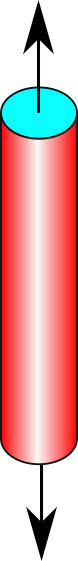
\includegraphics[width=\textwidth]{figs/hookes-law.png}
	\end{figure}
\end{minipage}	
\end{frame}

%----------------------------------------------------------------------------------------
\begin{frame}
\frametitle{Hooke's law}

\begin{equation*}
	\begin{Bmatrix}
		\varepsilon_{11}\\
		\varepsilon_{22}\\
		\varepsilon_{33}\\
	\end{Bmatrix} = \frac{1}{E}
	\begin{bmatrix}
		1 & -\nu & -\nu \\
		-\nu & 1 & -\nu \\
		-\nu & -\nu & 1 \\
	\end{bmatrix}
	\begin{Bmatrix}
		\sigma_{11}\\
		\sigma_{22}\\
		\sigma_{33}\\
	\end{Bmatrix}
\end{equation*}

It is possible to invert the matrix to obtain the generalized Hooke's law: \mode<beamer>{$[\sigma] = [\mathbf{C}][\varepsilon]$.}

\begin{equation*}
	\begin{Bmatrix}
		\sigma_{11}\\
		\sigma_{22}\\
		\sigma_{33}\\
		\sigma_{12}\\
		\sigma_{13}\\
		\sigma_{23}\\
	\end{Bmatrix} = \alpha
	\begin{bmatrix}
		(1-\nu) & \nu & \nu & 0 & 0 & 0 \\
	   			& (1-\nu) & \nu & 0 & 0 & 0 \\
	   			&  & (1-\nu) & 0 & 0 & 0 \\
	   			&  & & \frac{(1-2\nu)}{2} & 0 & 0 \\
	   			&  & & & \frac{(1-2\nu)}{2}  & 0 \\
	   			&  & & & & \frac{(1-2\nu)}{2} \\
	\end{bmatrix}
	\begin{Bmatrix}
		\varepsilon_{11}\\
		\varepsilon_{22}\\
		\varepsilon_{33}\\
		2\varepsilon_{12}\\
		2\varepsilon_{13}\\
		2\varepsilon_{23}\\
	\end{Bmatrix}
\end{equation*}
Where $\alpha = E / ((1+\nu)(1-2\nu))$.
Similarly, we can obtain the inverse matrix.
\end{frame}


%----------------------------------------------------------------------------------------
\begin{frame}
\frametitle{Hooke's law}
The matrices $[\mathbf{C}]$ and $[\mathbf{D}]$ contains two indepdent variables $E$ and $\mu$, where $E > 0$ and $-1 \le \mu \le 0.5$. 
The matrix can also be defined in terms of Lame's constants.
\begin{equation*}
	\begin{cases}
		\lambda = \frac{E \nu}{(1+\nu)(1-2\nu)} \quad \text{Lame's modulus (wave propagation)}\\
		\mu = G = \frac{E}{2(1+\nu)}
		\quad \text{Shear modulus (shear behavior)}\\
		K = \frac{E}{3(1-2\nu)}
		\quad \text{Bulk modulus (volumetric behavior)}\\
	\end{cases}
\end{equation*}
\end{frame}

%----------------------------------------------------------------------------------------
\begin{frame}
\frametitle{Isotropic linear elastic}
	\begin{figure}
		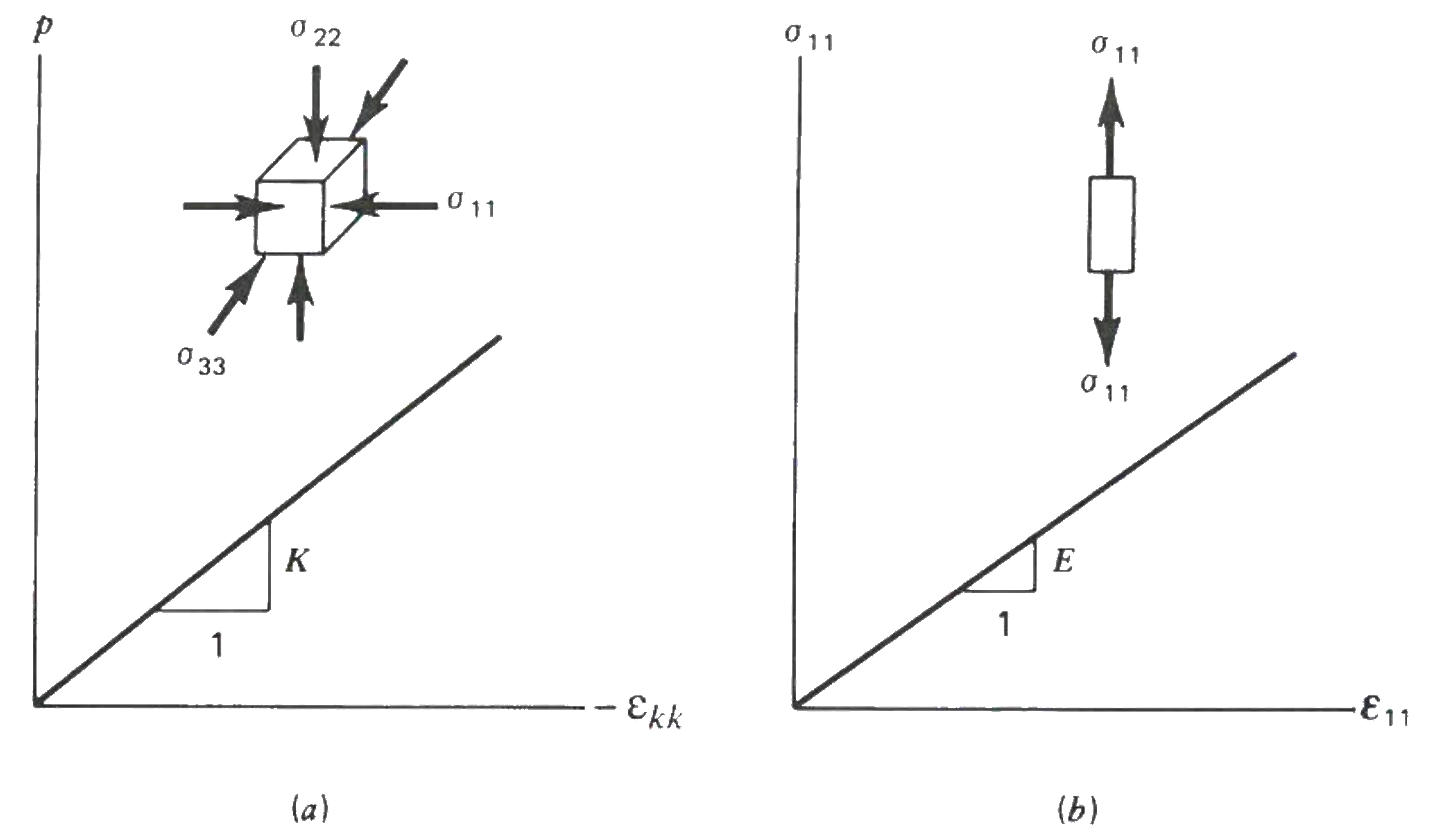
\includegraphics[width=0.95\textwidth]{figs/isotropic-linear-elastic.png}
		\caption*{Behavior of isotropic linear elastic material in simple tests: (a) hydrostatic compression test ($\sigma_{11} = \sigma_{22} = \sigma_{33} = p$) and (b) simple tension test (Chen 1994)}
	\end{figure}
\end{frame}

%----------------------------------------------------------------------------------------
\begin{frame}
\frametitle{Isotropic linear elastic}
\textbf{Hydrostatic compression test}
The non-zero components of stress: \mode<beamer>{$\sigma_{11} = \sigma_{22} = \sigma_{33} = -p = \sigma_{kk}/3$.}

The \textit{Bulk modulus, K,}  is defined as the ratio between the \textit{hydrostatic pressure p} nd the corresponding volume change $\delta \varepsilon_v = \varepsilon_{kk}$. 
\mode<beamer>{	
	\begin{equation*}
		K = - \frac{p}{\varepsilon_{kk}} = \lambda + \frac{2}{3}\mu
	\end{equation*}
}  
\mode<handout>{
	\vspace{1.5cm}
} 
\textbf{Simple tension test}
The only non-zero components of stress: \mode<beamer>{$\sigma_{11} = \sigma$}

The \textit{Young's modulus, E,}  and \textit{Poisson's ratio, $\nu$} as. 
\mode<beamer>{	
	\begin{equation*}
	E = \frac{\sigma_{11}}{\varepsilon_{11}} \quad
	\nu = \frac{-\varepsilon_{22}}{\varepsilon_{11}} = \frac{-\varepsilon_{33}}{\varepsilon_{11}}
	\end{equation*}
}  
\mode<handout>{
	\vspace{1.5cm}
}
\end{frame}

%----------------------------------------------------------------------------------------
\begin{frame}
\frametitle{Isotropic linear elastic}
\begin{figure}
	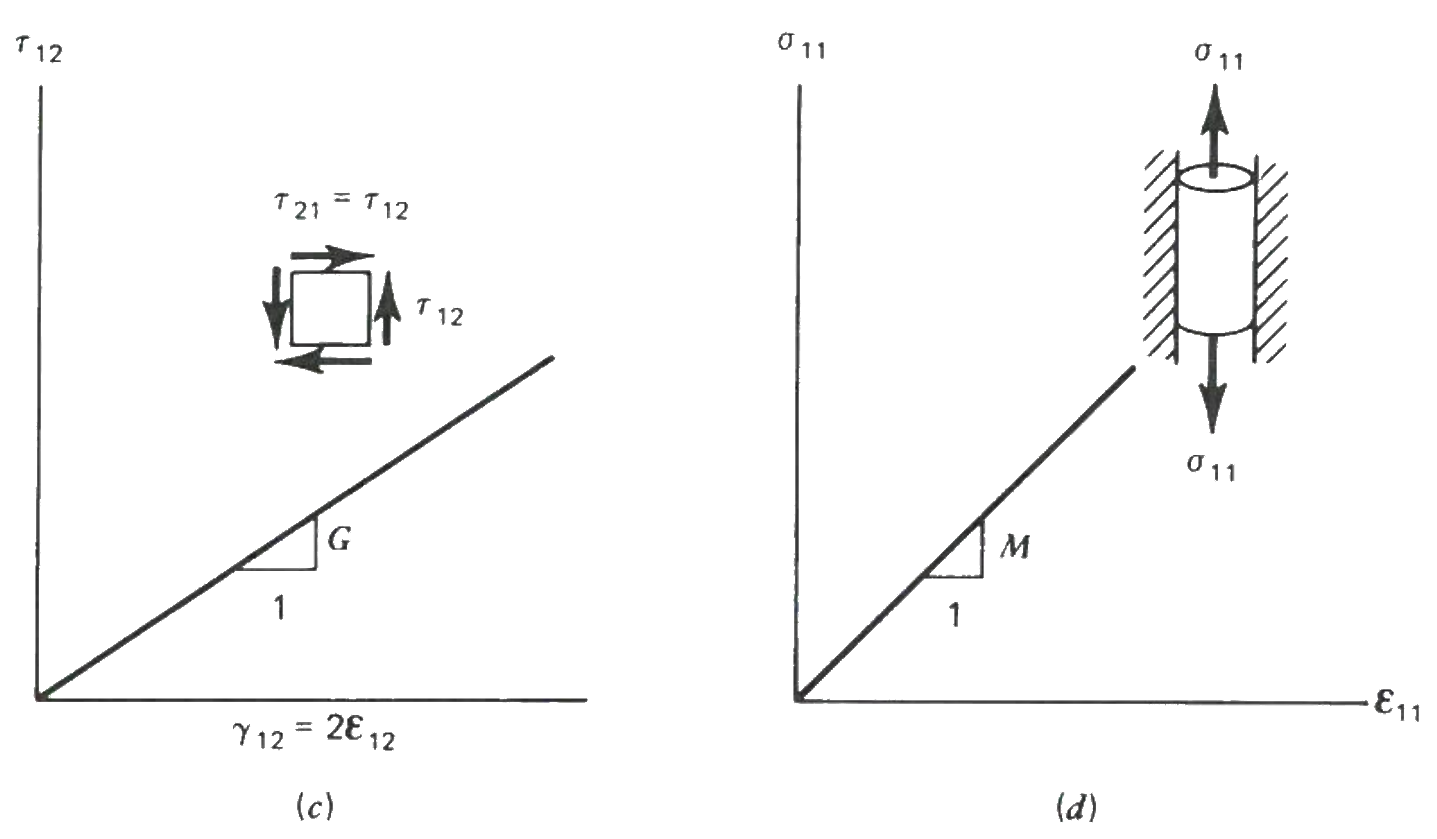
\includegraphics[width=0.95\textwidth]{figs/isotropic-linear-elastic-1.png}
	\caption*{Behavior of isotropic linear elastic material in simple tests: (c) pure shear test, and (d) uniaxial strain test (Chen 1994)}
\end{figure}
\end{frame}

%----------------------------------------------------------------------------------------
\begin{frame}
\frametitle{Isotropic linear elastic}
\textbf{Simple shear test}

The non-zero components of stress: \mode<beamer>{$\sigma_{12} = \sigma_{21} = \tau_{12} = \tau_{21} = \tau$.}

The \textit{Shear modulus, $G$ or $\mu$,}  is defined as: 
\mode<beamer>{	
	\begin{equation*}
	G = \mu = \frac{\sigma_{12}}{\gamma_{12}} = \frac{\tau}{2\varepsilon_{12}}
	\end{equation*}
}  
\mode<handout>{
	\vspace{1.5cm}
}

\textbf{Uniaxial strain test}
The test is carried out by applying a uniaxial stress component $\sigma_{11}$ in the axial direction of a cylindrical sample, whose lateral surface is \textit{restrained} against lateral movement (Oedometer test). Axial strain $\varepsilon_{11}$ is the only nonvanishing component. The \textit{constrained modulus M} or as PLAXIS calls it $E_{oed}$ is defined as the ratio between $\sigma_{11}$ and $\varepsilon_11$.
\mode<beamer>{	
	\begin{align*}
		\sigma_{11} & = \frac{E}{(1+\nu)(1-2\nu)}\left[(1-\nu)\varepsilon_{11} + \nu\cancelto{0}{\varepsilon_{22}} + \nu\cancelto{0}{\varepsilon_{33}}\right] = \frac{E(1-\nu)\varepsilon_{11}}{(1+\nu)(1-2\nu)} \\
		M & = E_{oed} = \frac{\sigma_{11}}{\varepsilon_{11}} = \frac{(1 - \nu)E}{(1+\nu)(1-2\nu)} = (\lambda + 2\mu)
	\end{align*}
}  
\mode<handout>{
	\vspace{1.5cm}
}

\end{frame}


%----------------------------------------------------------------------------------------
\begin{frame}
\frametitle{Plane stress v Plane strain}
For a frame with an axis perpendicular to the plane of interest, $x_3$ or $z$:

\textbf{Plane stress}
\mode<beamer>{$\sigma_{33} = \sigma_{zz} = \tau_{xz} = \tau_{yz} = 0$.}\mode<handout>{\vspace{1cm}.}

The strain in $z$ is written as:
\mode<beamer>{	
	\begin{equation*}
	\varepsilon_{zz} = \frac{-\nu}{E}(\sigma_{xx} + \sigma_{yy}) = \frac{-\nu}{1-\nu}(\varepsilon_{xx} + \varepsilon_{yy}) 
	\end{equation*}
The plane stress are commonly used for thin flat plates loaded in the plane of the plate.
}  
\mode<handout>{
	\vspace{2.5cm}
}


\textbf{Plane strain}
\mode<beamer>{$\varepsilon_{33} = \varepsilon_{zz} = \gamma_{xz} = \gamma_{yz} = 0$.}\mode<handout>{\vspace{1cm}.}

The stress in $z$ is written as:
\mode<beamer>{	
	\begin{equation*}
	\sigma_{zz} = \nu(\sigma_{xx} + \sigma_{yy})
	\end{equation*}
	The plane strains are commonly used for elongated bodies of uniform cross sections subjected to uniform loading along the longitudinal axis (tunnels, dams, retaining walls, soil slopes, etc.).
}  
\mode<handout>{
	\vspace{2.5cm}
}
\end{frame}


%----------------------------------------------------------------------------------------
\begin{frame}
\frametitle{Elastic solutions}
\mode<beamer>{	
	\begin{enumerate}
		\item \textit{Ease of use} Only two parameters, choose equivalent values representative of stran/stress levels.
		\item \textit{Disadvantage}: No failure criteria.
		\item Validate code with chart solutions ("\textit{Exact solutions}")., e.g., Poulos and Davis (1974).
		\item Useful to get feeling of problem (lo stress levels) not wide distribution of plastic zones.
	\end{enumerate}
}  
\mode<handout>{
	\vspace{6cm}
}
\end{frame}

%------------------------------------------------
\begin{frame}
\frametitle{Pore-pressure analysis in geotechnical engineering}
\begin{figure}[ht]
	\centering
	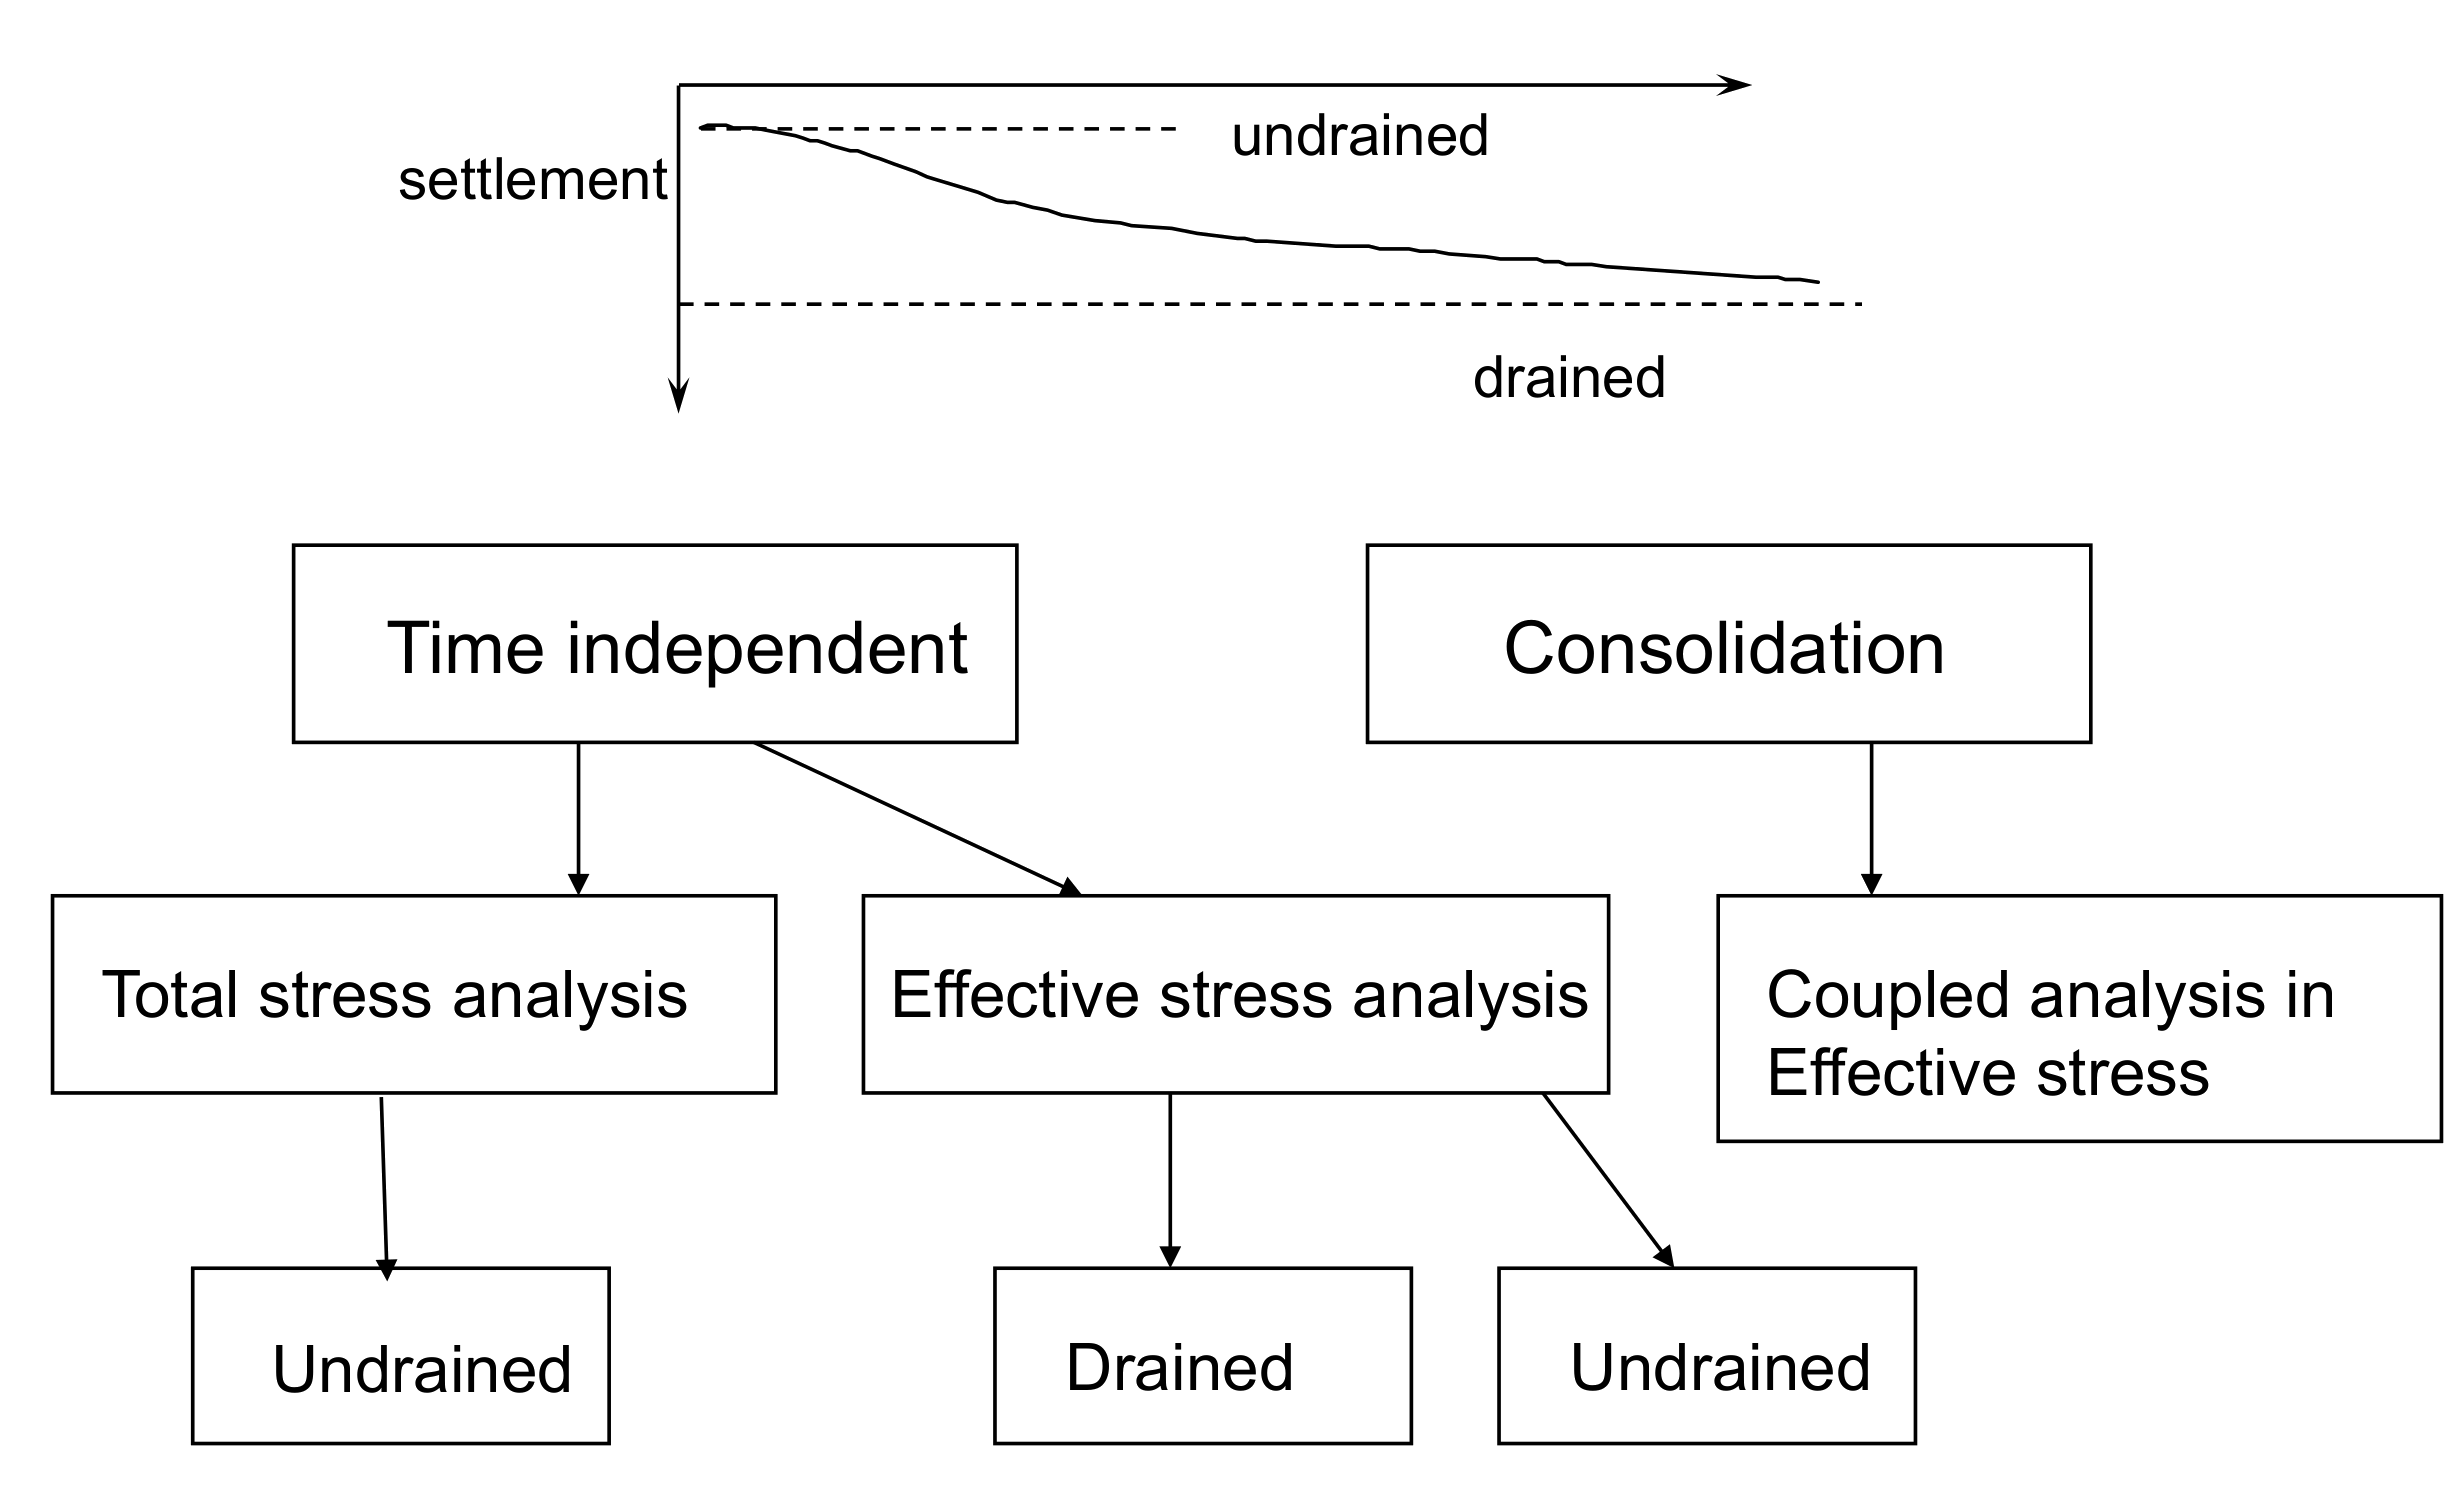
\includegraphics[width=\textwidth]{figs/geotechnical-analysis.png}
\end{figure}
\end{frame}

%------------------------------------------------

\begin{frame}
\frametitle{Drained analysis - Effective stress}
\begin{enumerate}
	\item Need to assign initial effective stresses before the analysis.
	\item Can use any effective stress model: Elastic, Mohr-Coulomb/Drucker Prager and Cam-Clay models.
	\item If plasticity models are used, need to update the effective stresses at each increment:
	\mode<beamer>{
		\begin{equation*}
			\sigma^\prime(new) = \sigma^\prime(old) + D(\text{soil skeleton}) d\varepsilon
		\end{equation*}
	}
	\mode<handout>{	
		\vspace{1.5cm}
	}
	\item Very common.
\end{enumerate}
\end{frame}

%------------------------------------------------
\begin{frame}
\frametitle{Undrained analysis - Total stress}
\begin{itemize}
	\item Excess pore pressure cannot be calculated. 
	\item Effective stress state of the soil cannot be examined.
	\item Elastic model is commonly used for deformation
	\mode<beamer>{
		\begin{enumerate}
			\item Use undrained stiffness $E_u$ and strength parameters $s_u$
			\item Poisson's ratio close to 0.5 with a drained simulation
			\item Properties can vary with depth. ($K_0$ varies)
			\item Consolidation analysis has no effect and should not be performed.
		\end{enumerate}
	}
	\mode<handout>{
		\vspace{2.5cm}
	}
	\item Von-Mises model is used for modeling undrained shear strength of clays. ($C_u$ or $s_u$ and undrained friction $\phi_u = 0$)
	\item Can assign different stiffness and strength at different depths explicity by assigning different model parameters at different depths.
\end{itemize}
\end{frame}

%------------------------------------------------
\begin{frame}
\frametitle{Undrained analysis - Effective vs Total stress}
\mode<beamer>{
	\begin{itemize}
		\item Effective stress: $E^\prime$ and $\nu^\prime$.
		\item Total stress: $E_u$ and $\nu_u$
		\item No volume change:
			\begin{equation*}
				\nu_u = 0.5; (K_u = E_u/(1-2\nu_u)/3 = E_u / 0 = \infty)
			\end{equation*}
		\item Pore fluid cannot sustain shear stresses. Soil skeleton carries the shear stresses $\tau (or q)$.
		\begin{align*}
			G^\prime = G_u; \quad G^\prime & = E^\prime / (1+\nu^\prime)/2 \quad G_u = E_u /(1+\nu_u)/2\\
			E^\prime/(1+\nu^\prime)/2 & = E_u /(1+ 0.5)/2\\
			E_u & = 1.5 E^\prime /(1+\nu^\prime)
		\end{align*}
		\item In finite element analysis, $\nu_u = 0.5$ cannot be used. Use $\nu_u = 0.49 \text{ or } 0.495$. But be careful with \textit{mesh locking} problem.
	\end{itemize}
}
\end{frame}

%------------------------------------------------
\begin{frame}
\frametitle{Undrained analysis - Effective stress}
\begin{itemize}
	\item Need to assign initial effective stresses before the analysis.
	\item Can use any effective stress model, so the stiffness and strength variation with depth can be modeled implicitly with the one set of model parameters.
	\item The applied load is carried by the soil skeleton and pore water.
	\item The contribution of the bulk modulus of water needs to be added:
	\mode<beamer>{
		\begin{equation*}
		D = D_{(\text{soil skeleton})} + \frac{1}{n}D_{(water)}, \quad \text{where \textit{n} is the porosity}
		\end{equation*}
	}
	\mode<handout>{
		\vspace{1cm}
	}
	\item Effective stress increment can be computed by:
	\mode<beamer>{
		\begin{equation*}
			d\sigma^\prime = D_{(\text{soil skeleton})} d\varepsilon.
		\end{equation*}
	}
	\mode<handout>{
		\vspace{1cm}
	}
	\item Need to update the effective stresses at each time step.
\end{itemize}
\end{frame}

\note{
	\begin{equation*}
		u = K_w \cdot \varepsilon_{v, water}
	\end{equation*}
	
	Where, $K_w$ is the Bulk modulus of water $\approx 2 \times 10^6 kN/m^2$. 
	
	\begin{align*}
		\varepsilon_{v, water} &= \Delta V_w / V_w \\
		\varepsilon_{v, soil} &= \Delta V_T / V_T  = \Delta V_w / V_T \quad \text{(assuming solid is incompressible)}\\
		\frac{\varepsilon_{v, soil}}{\varepsilon_{v, water}}  & = \frac{\Delta V_w / V_T}{\Delta V_w / V_w} = \frac{V_w}{V_T} = n \quad \text{(porosity for s = 100\%)}
	\end{align*}

	Therefore,
	
	\begin{equation*}
		u = K_w \cdot \frac{\varepsilon_{v, soil}}{n} = (K_w / n) \cdot \varepsilon_{v, soil}
	\end{equation*}
}

\note{
	Consider equivalent $(K_w/n)$ in soil model. Separate total and effective stresses:
	
	\begin{align*}
		\sigma_m & = K_u \cdot \varepsilon_{v, soil} \quad K_u \text{undrained bulk modulus of soil} \\
		\sigma_m^\prime & = K^\prime \cdot  \varepsilon_{v} \\
		u & = \sigma_m - \sigma^\prime = (K_u - K^\prime) \cdot  \varepsilon_v\\
		K_w/n & = K_u - K^\prime
	\end{align*}
}

\note{
	\begin{figure}
		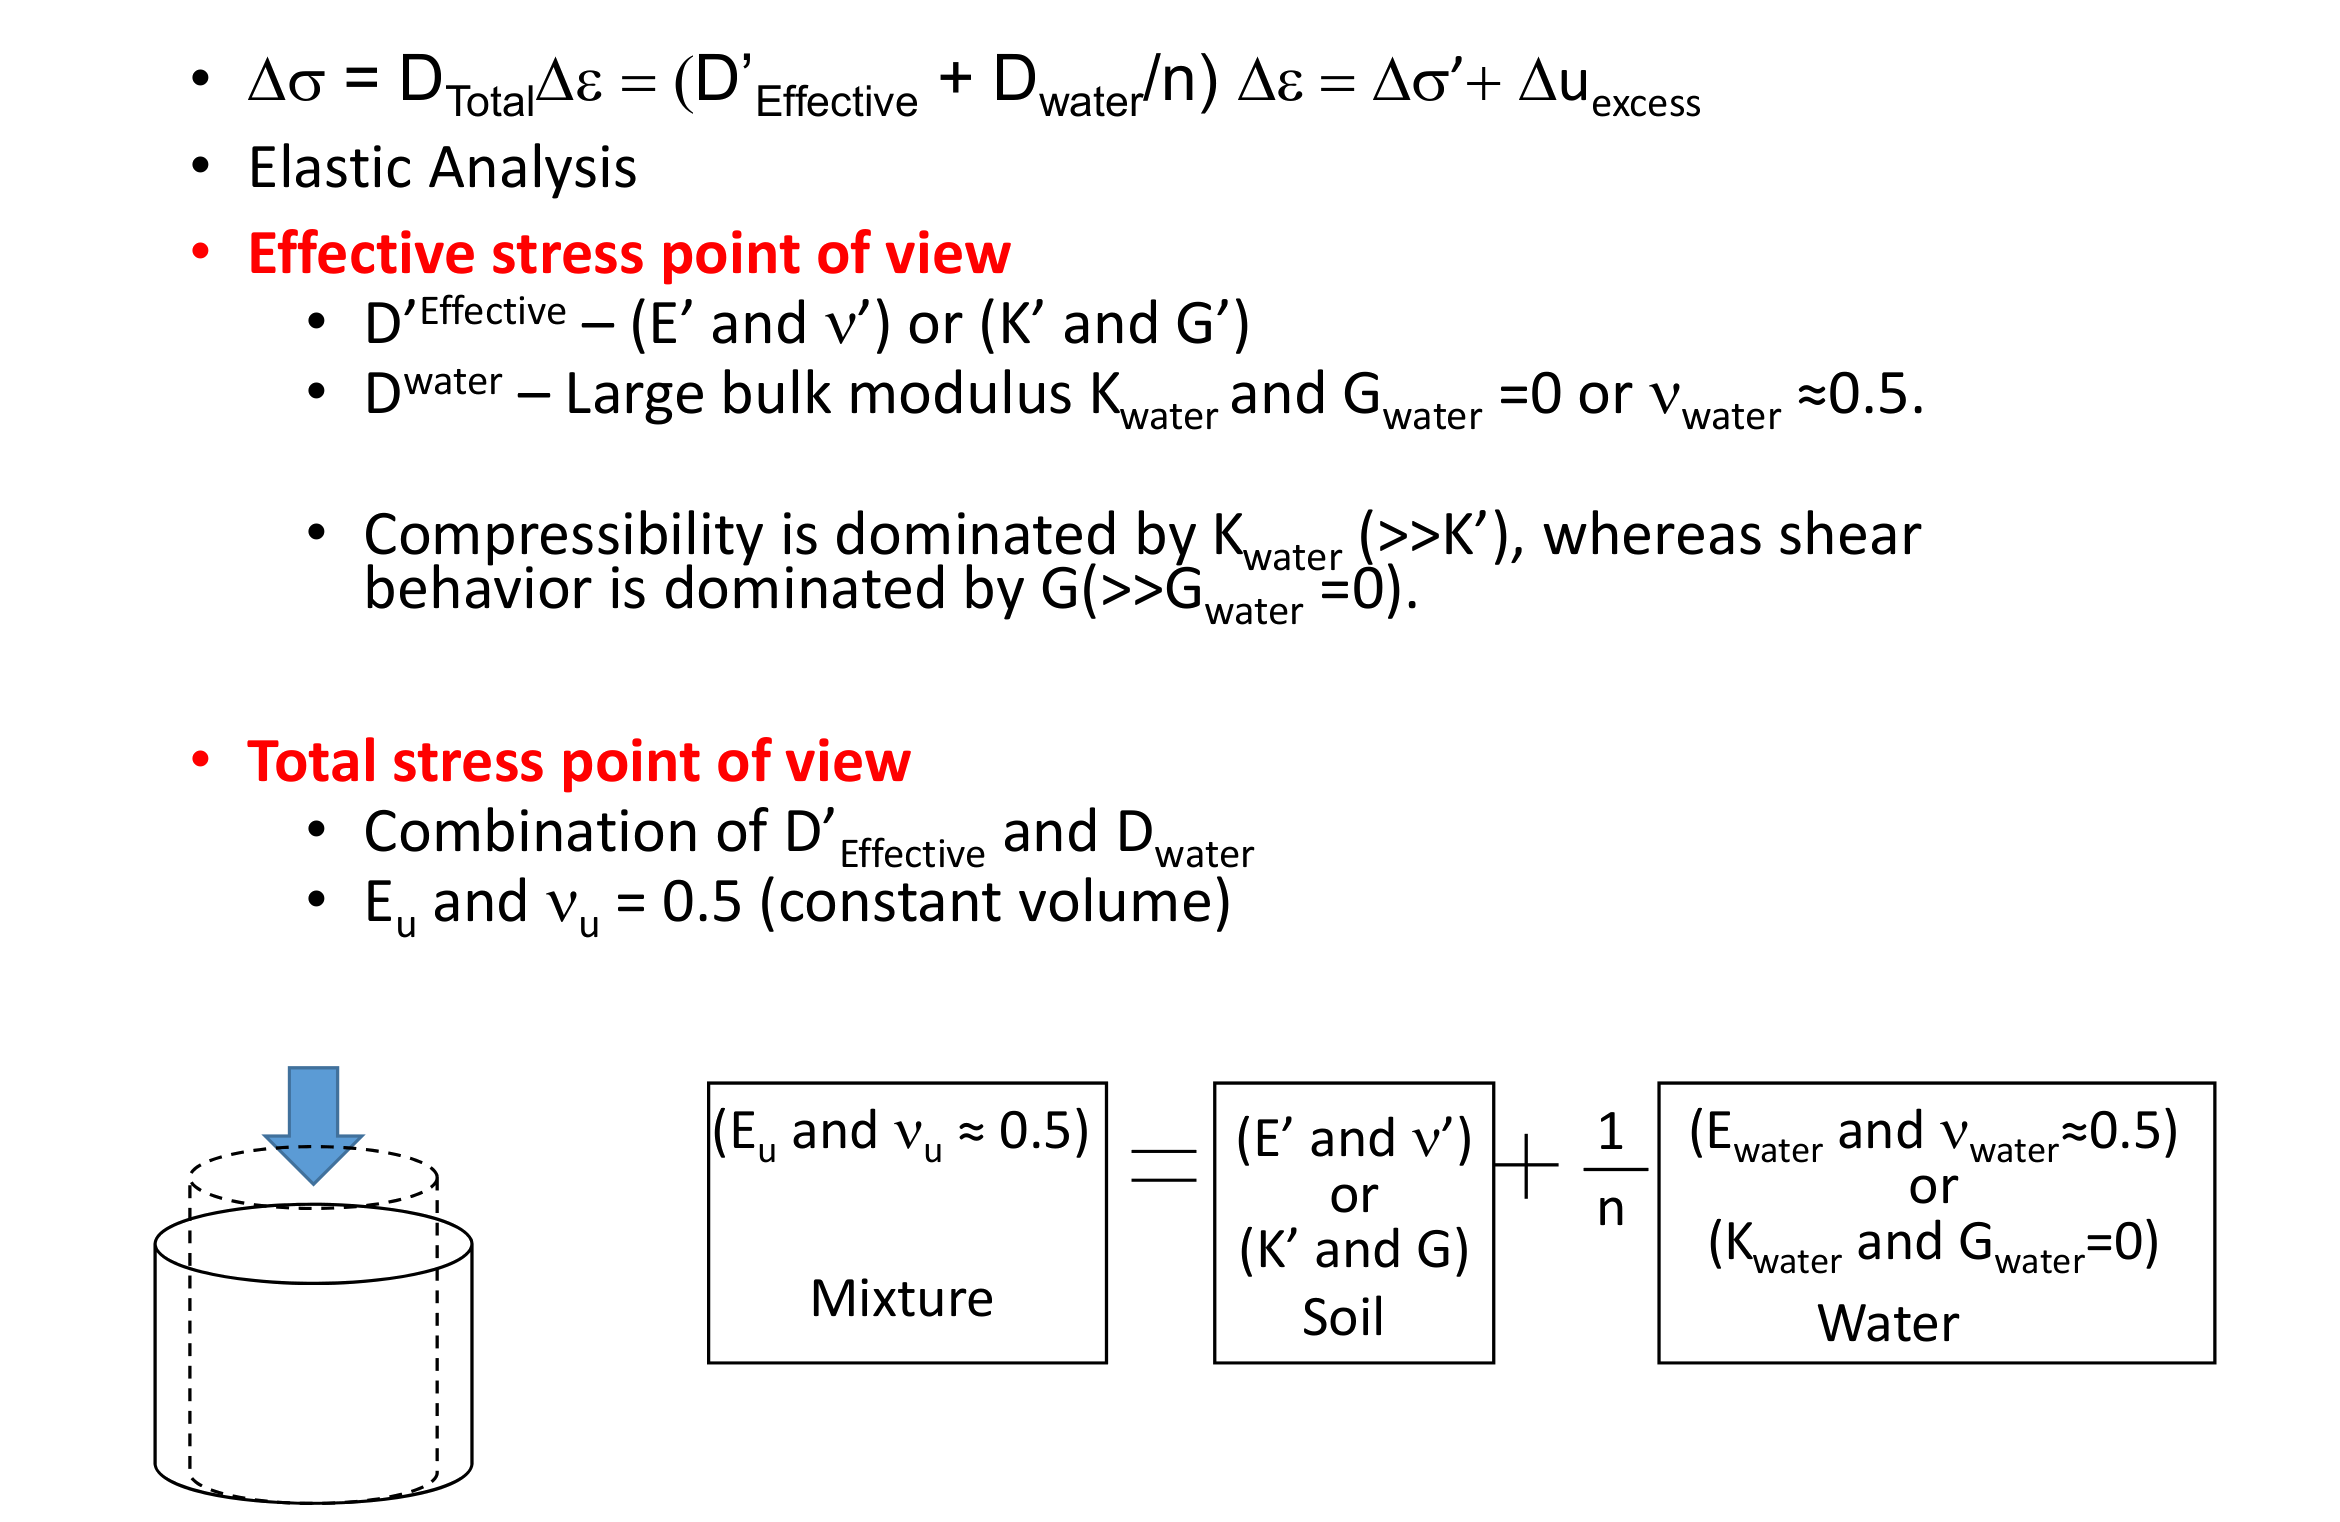
\includegraphics[width=0.8\textwidth]{figs/undrained-test.png}
	\end{figure}
}

%------------------------------------------------
\begin{frame}
\frametitle{Effective stress approach or undrained (A)}
\begin{itemize}
	\item Effective stiffness and effective strength parameters are used.
	\item \textit{Pore pressures are generated}, but may be \textbf{inaccurate} depending on the model.
	\item Undrained shear strength is \textit{not} an input parameter but an outcome of the constitutive model. The resulting shear strength must be checked against known data!
	\item Consolidation analysis can be performed after the undrained calculation, which \textit{affects the shear strength}!
\end{itemize}
\end{frame}

%------------------------------------------------
\begin{frame}
\frametitle{Equivalent effective stress approach or undrained (B)}
\begin{itemize}
	\item Effective stiffness parameters and \textit{undrained strength parameters }are used.
	\item \textit{Pore pressures are generated}, but may be hightly \textbf{inaccurate}.
	\item Undrained shear strength is an input parameter.
	\item Consolidation analysis should not be performed after the undrained calculation, $s_u$ must be updated, if consolidation is performed anyway!
\end{itemize}
\end{frame}


%------------------------------------------------
\begin{frame}
\frametitle{Methods of undrained analysis for Mohr-Coulomb clay}
\begin{table}
	\begin{tabularx}{\textwidth}{XXXXX}
		\toprule
		\textbf{undrained analysis}          & \textbf{material type} & \textbf{deformation parameters} & \textbf{strength parameters} & \textbf{initial conditions} \\
		\midrule
		\textbf{Total stress}                           & Non-porous / drained   & $E_u, \nu_u$                    & $c_u, \phi_u = 0$            & $K_{0,u}$                   \\
		\midrule 
		\textbf{Effective stress} & Undrained (triaxial parameters)             & $E^\prime, \nu^\prime$          & $c^\prime, \phi^\prime$      & $K_0$                       \\
		\midrule
		\textbf{Equivalent Effective stress}    & Undrained (strength profile)           & $E^\prime, \nu^\prime$          & $c^\prime, \phi^\prime$      & $K_0$ \\    
		\bottomrule                 
	\end{tabularx}
\end{table}
\end{frame}

%------------------------------------------------
\begin{frame}
\frametitle{Consolidation analysis - Effective stress}
\begin{itemize}
	\item Use Biot's 3D consolidation theory
	\item Pore pressure and displacement are computed at each time step.
	\item Need to use effective stress model
	\item Need permeability
	\item Lots of computational time
	\item More realistic. Undrained, partially drained, drained depending on the loading condition, drainage condition, permeability of soil.
	\item Stress path followed is correct, which should provide a good strain estimate when plasticity models are used.
\end{itemize}
\end{frame}

%----------------------------------------------------------------------------------------
\section{Project on FEA of an excavation}
%----------------------------------------------------------------------------------------
\begin{frame}
\frametitle{Total stress evaluating varying $K_0$}
\begin{figure}
	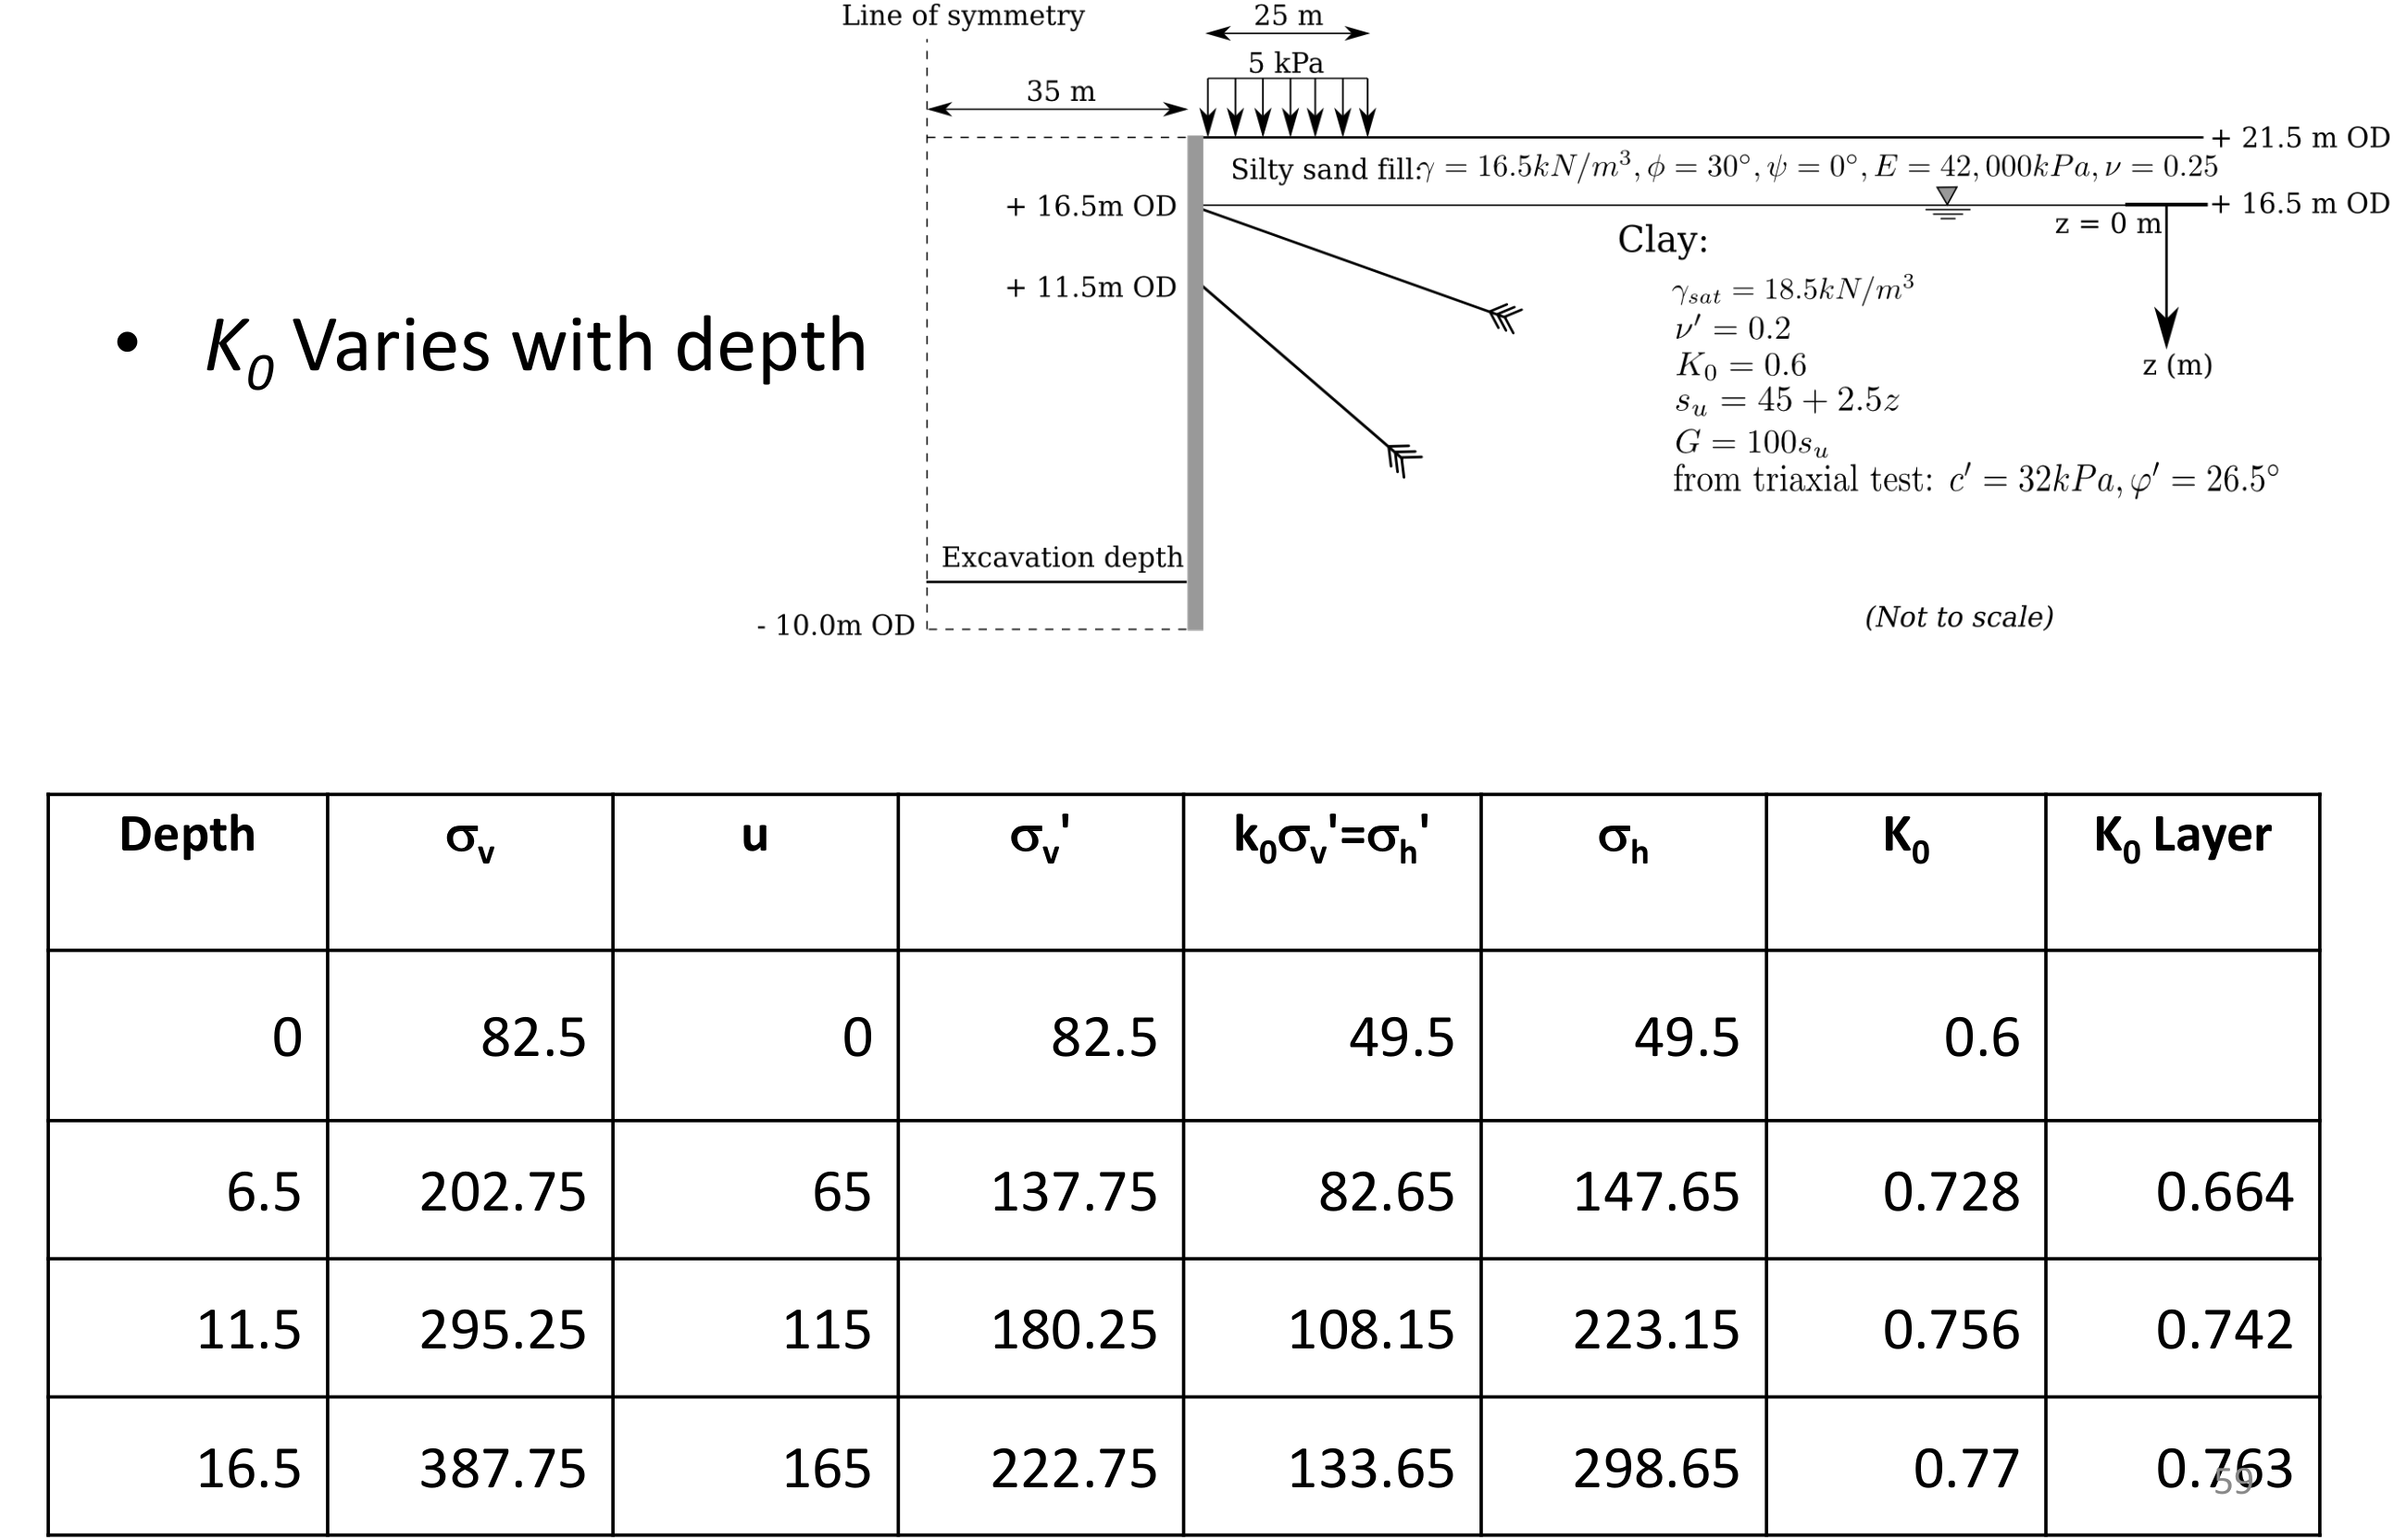
\includegraphics[width=0.95\textwidth]{figs/excavation-k0.png}
\end{figure}
\end{frame}

%----------------------------------------------------------------------------------------
\begin{frame}
\frametitle{Undrained analysis using effective stress method}
\textbf{Effective stress Method A}
\begin{itemize}
	\item Define $c^\prime$ and $\phi^\prime$ in terms of the real effective stress parameters, assuming zero dilation.
	\item $\nu^\prime$ is the effective Poisson ratio
	\item $E$ and $K_0$ should be `\textit{effective stress}' based.
\end{itemize}
\begin{figure}
	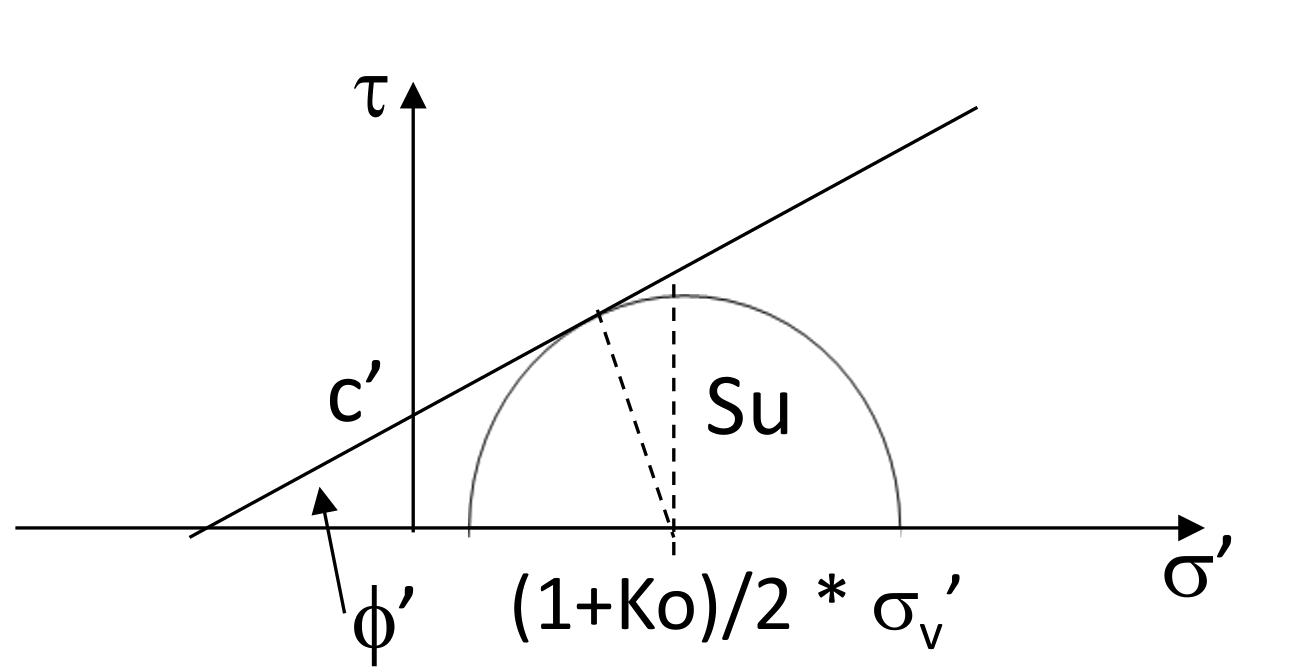
\includegraphics[width=0.6\textwidth]{figs/su-effective.png}
	\caption*{Mohr-Coulomb failure criteria: $\tau = c^\prime + \sigma^\prime \tan \phi^\prime$}
\end{figure}
	\begin{equation*}
		s_u = c^\prime \cos \phi^\prime + (1+K_0)/2 \cdot \sin \phi^\prime \cdot \sigma_{v0}^\prime.
	\end{equation*}
\end{frame}

%----------------------------------------------------------------------------------------
\begin{frame}
\frametitle{Undrained analysis using equivalent effective stress method}
\textbf{Effective stress Method B}
\begin{itemize}
	\item Define $c^\prime$ and $\phi^\prime$ in terms of the ``\textit{equivalent}'' effective stress parameters, with zero dilation. Parameters are defined based on the strength profile with depth.
	\item $\nu^\prime$ is the effective Poisson ratio
	\item $E$ and $K_0$ should be `\textit{effective stress}' based.
\end{itemize}
\begin{figure}
	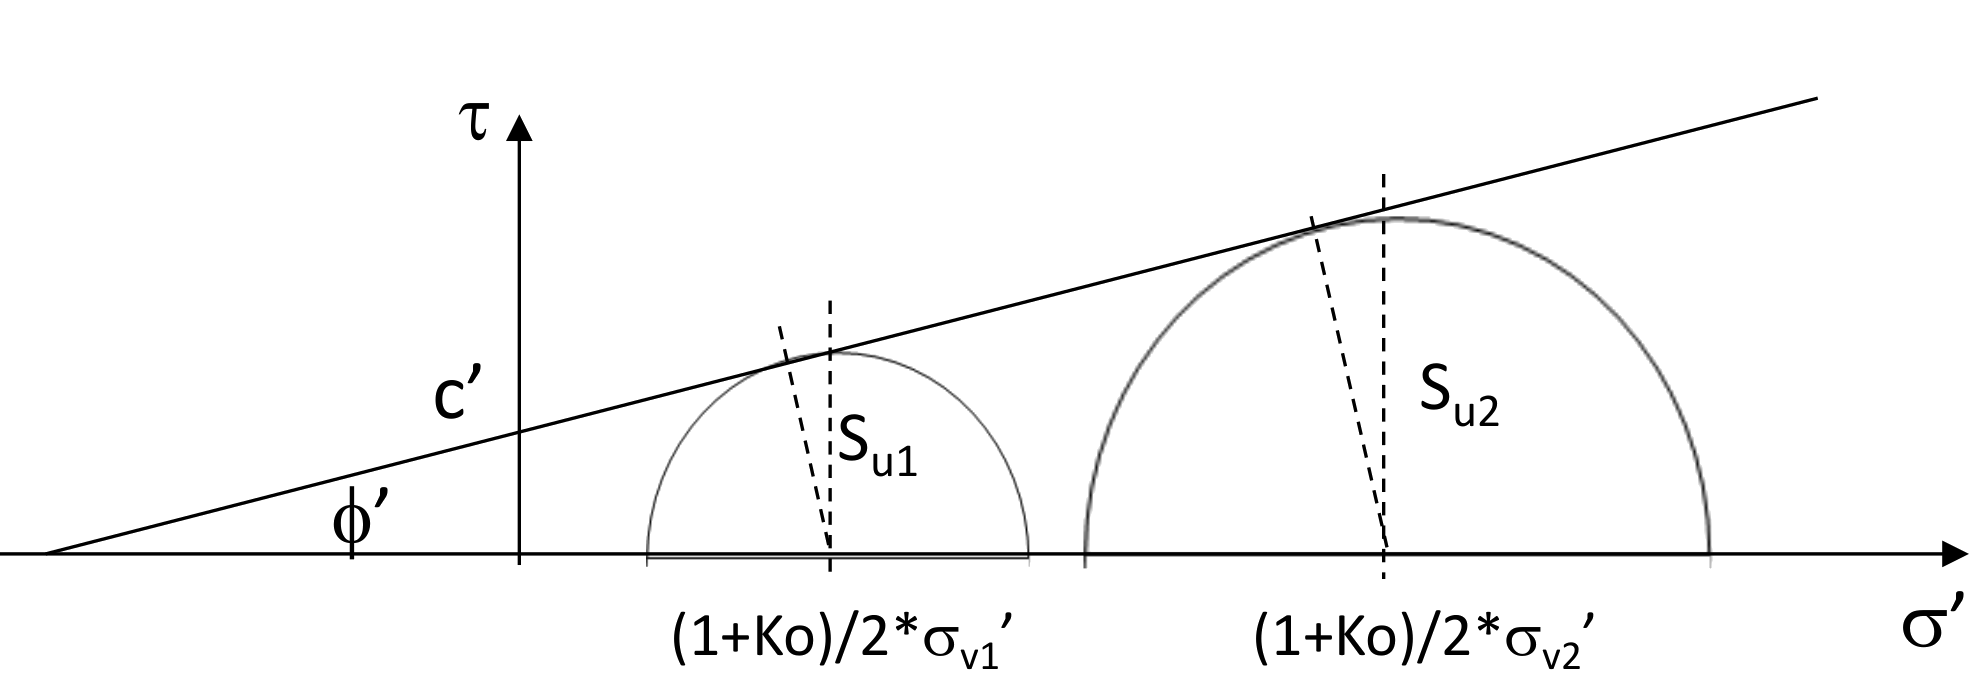
\includegraphics[width=0.6\textwidth]{figs/su-total.png}
	\caption*{Mohr-Coulomb failure criteria: $\tau = c^\prime + \sigma^\prime \tan \phi^\prime$}
\end{figure}
\begin{equation*}
s_u = c^\prime \cos \phi^\prime + (1+K_0)/2 \cdot \sin \phi^\prime \cdot \sigma_{v0}^\prime.
\end{equation*}
\end{frame}

%------------------------------------------------
\section{Slope stability}
%------------------------------------------------
\begin{frame}
\frametitle{2014 Oso landslide}
\begin{figure}[ht]
	\centering
	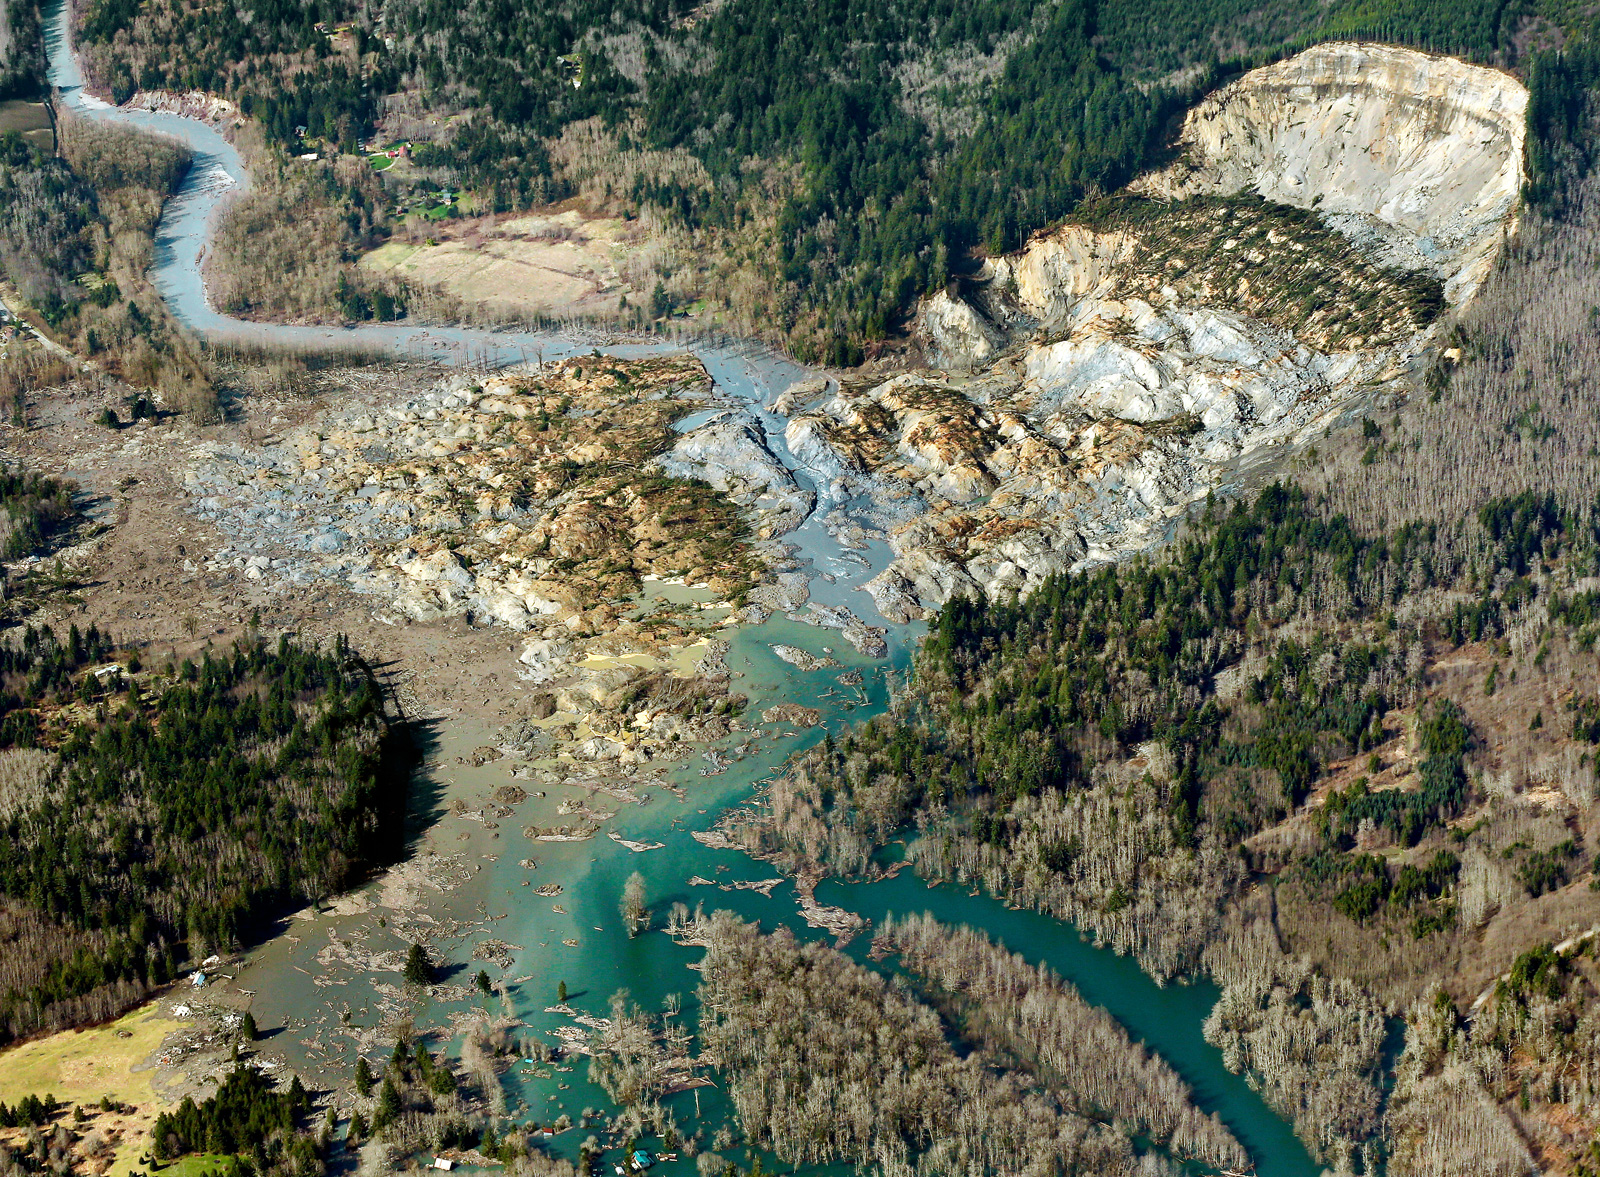
\includegraphics[width=\textwidth]{figs/oso-mudslide.jpg}
\end{figure}
\end{frame}

\note{
\begin{itemize}
	\item 22nd March 2014 at 10.37 am
	\item Volume: approx. 8 million m3
	\item 43 casualties (deadliest landslide in US)
	\item 1 neighboured destroyed
	\item \textbf{Cost unknown} but $>$ USD 150 million + USD 65 million (lawsuit 2017) + indirect costs
	\item Social tensions (general public \& sc. community)
	\item Indian Snohomish tribe
\end{itemize}
}

%------------------------------------------------
\begin{frame}
\frametitle{Shear failure plane}
\begin{figure}[ht]
\centering
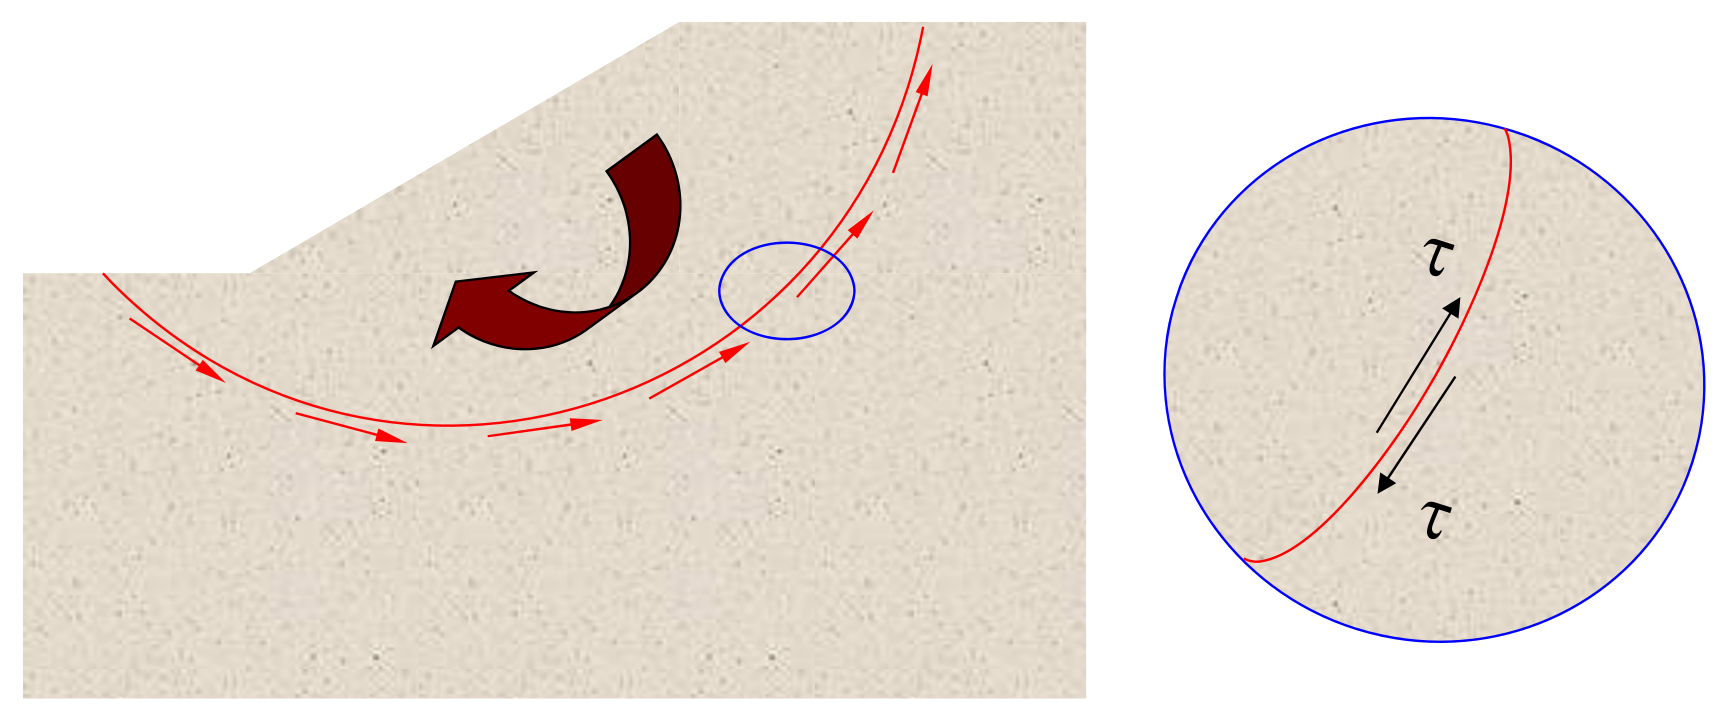
\includegraphics[width=0.9\textwidth]{figs/shear-failure-plane.png}
\caption*{At failure, shear stress along the failure surface ($\tau$) reaches the shear strength ($\tau_f$).}
\end{figure}
Factor of Safety = \mode<beamer>{Resistance (from soil shear strength)/Driving force (from total
stress equilibrium (i.e. weight of the soil))}
\end{frame}

%------------------------------------------------
\begin{frame}
\frametitle{Dry slope (total stress = effective stress)}
\mode<beamer>{
\begin{figure}[ht]
\centering
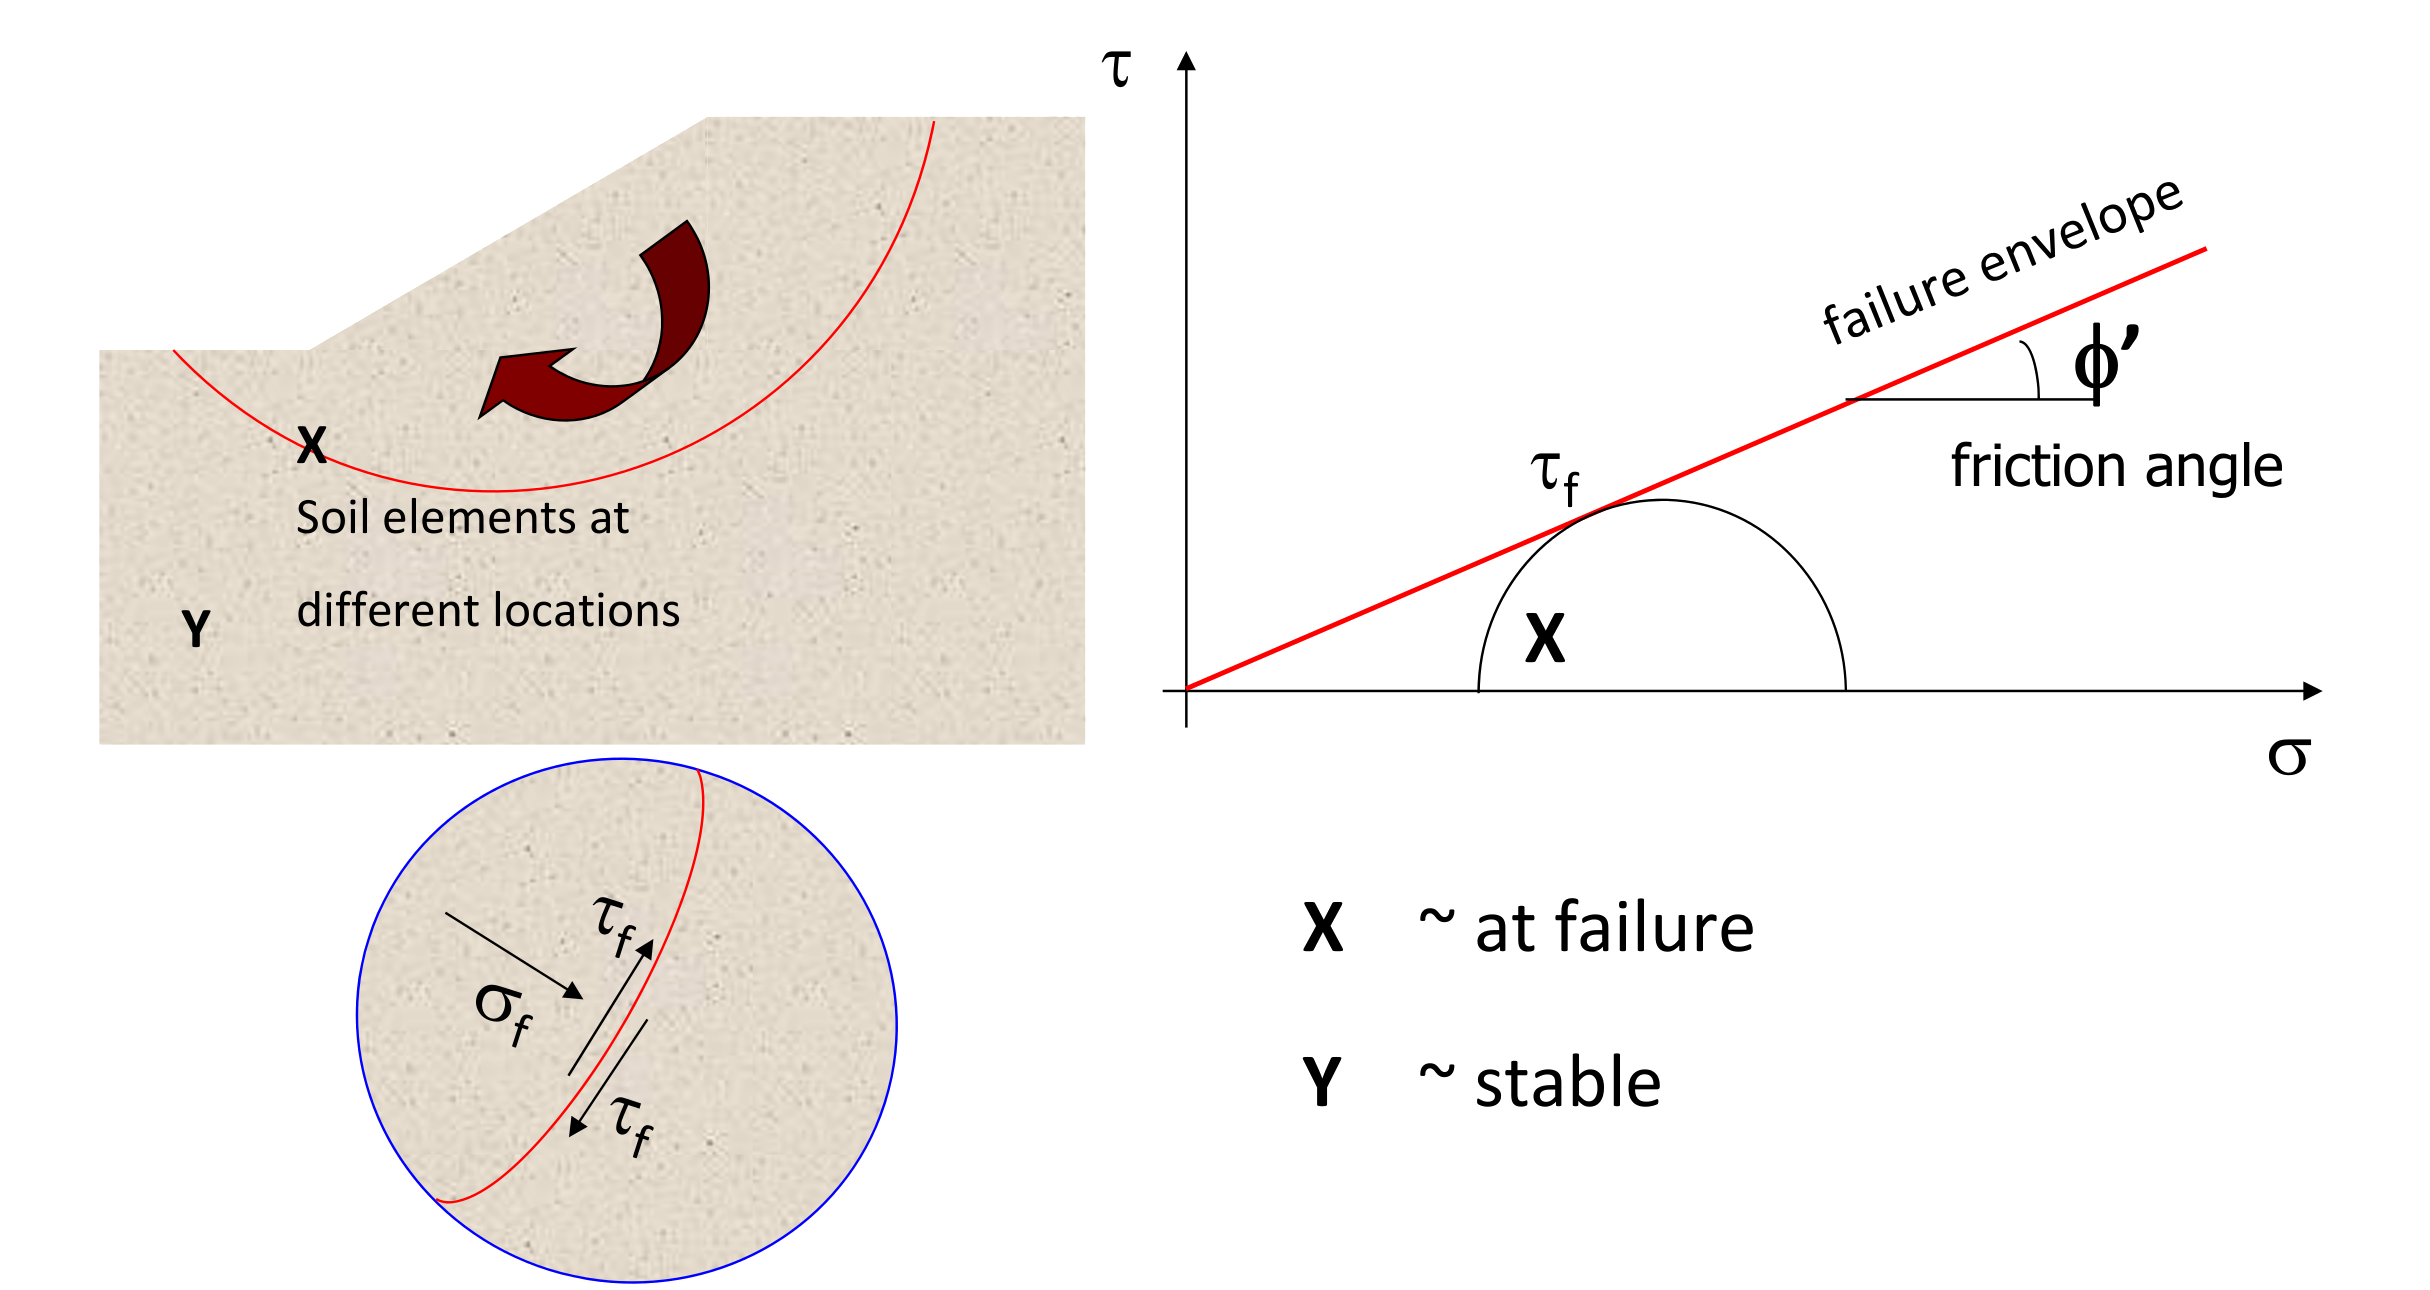
\includegraphics[width=\textwidth]{figs/dry-slope.png}
\end{figure}
}
\mode<handout>{
\begin{figure}[ht]
\centering
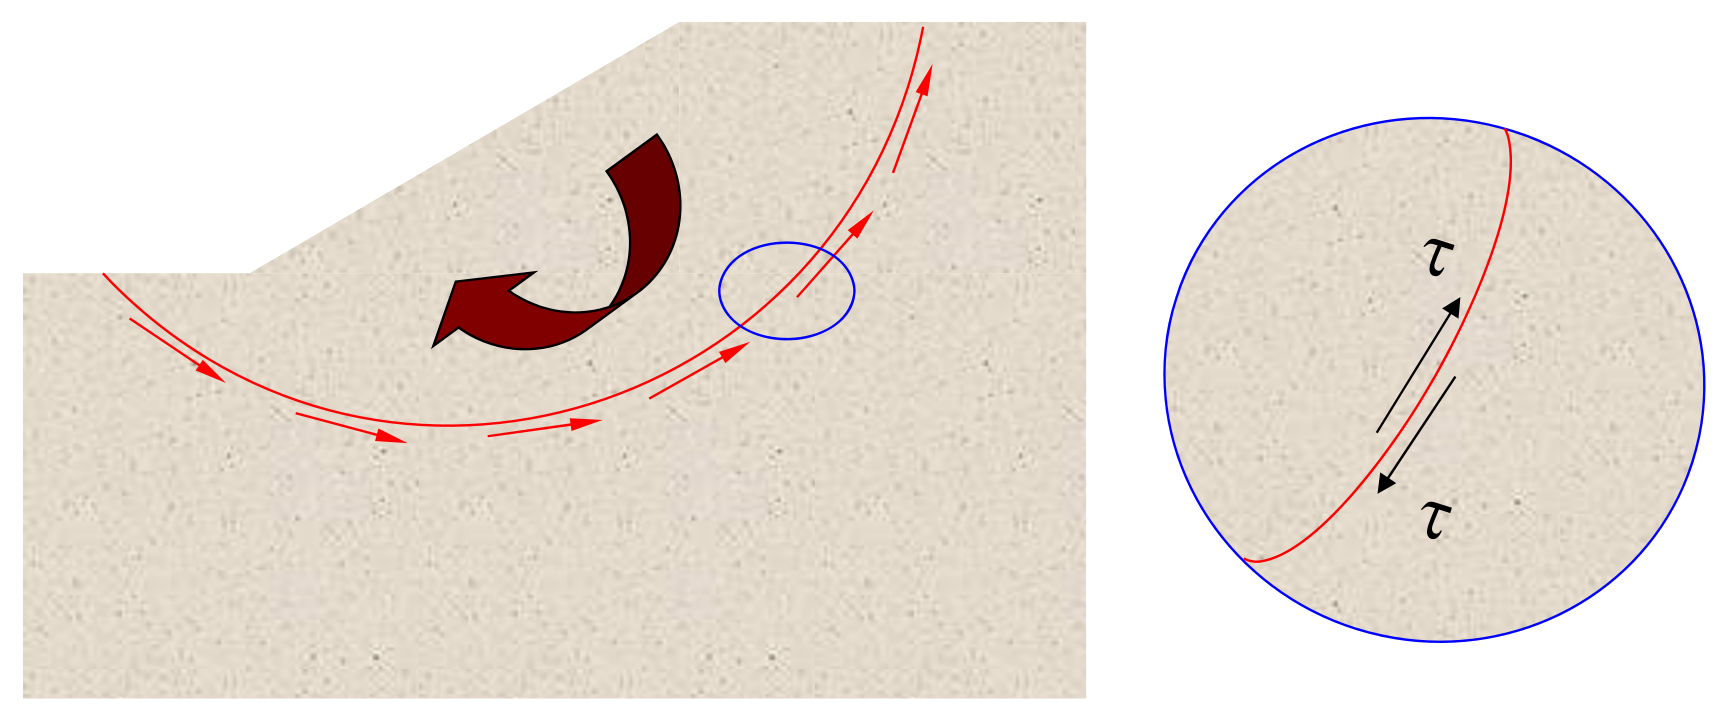
\includegraphics[width=0.9\textwidth]{figs/shear-failure-plane.png}
\end{figure}
}
\end{frame}

%------------------------------------------------
\begin{frame}
\frametitle{Saturated slope (total stress = effective stress + pwp)}
\textbf{Drained conditions} - need to compute the steady state pore pressure field
and then evaluate ``effective stress‐based'' shear strength to find the overall
stability (based on total stress equilibrium).
\mode<beamer>{
\begin{figure}[ht]
\centering
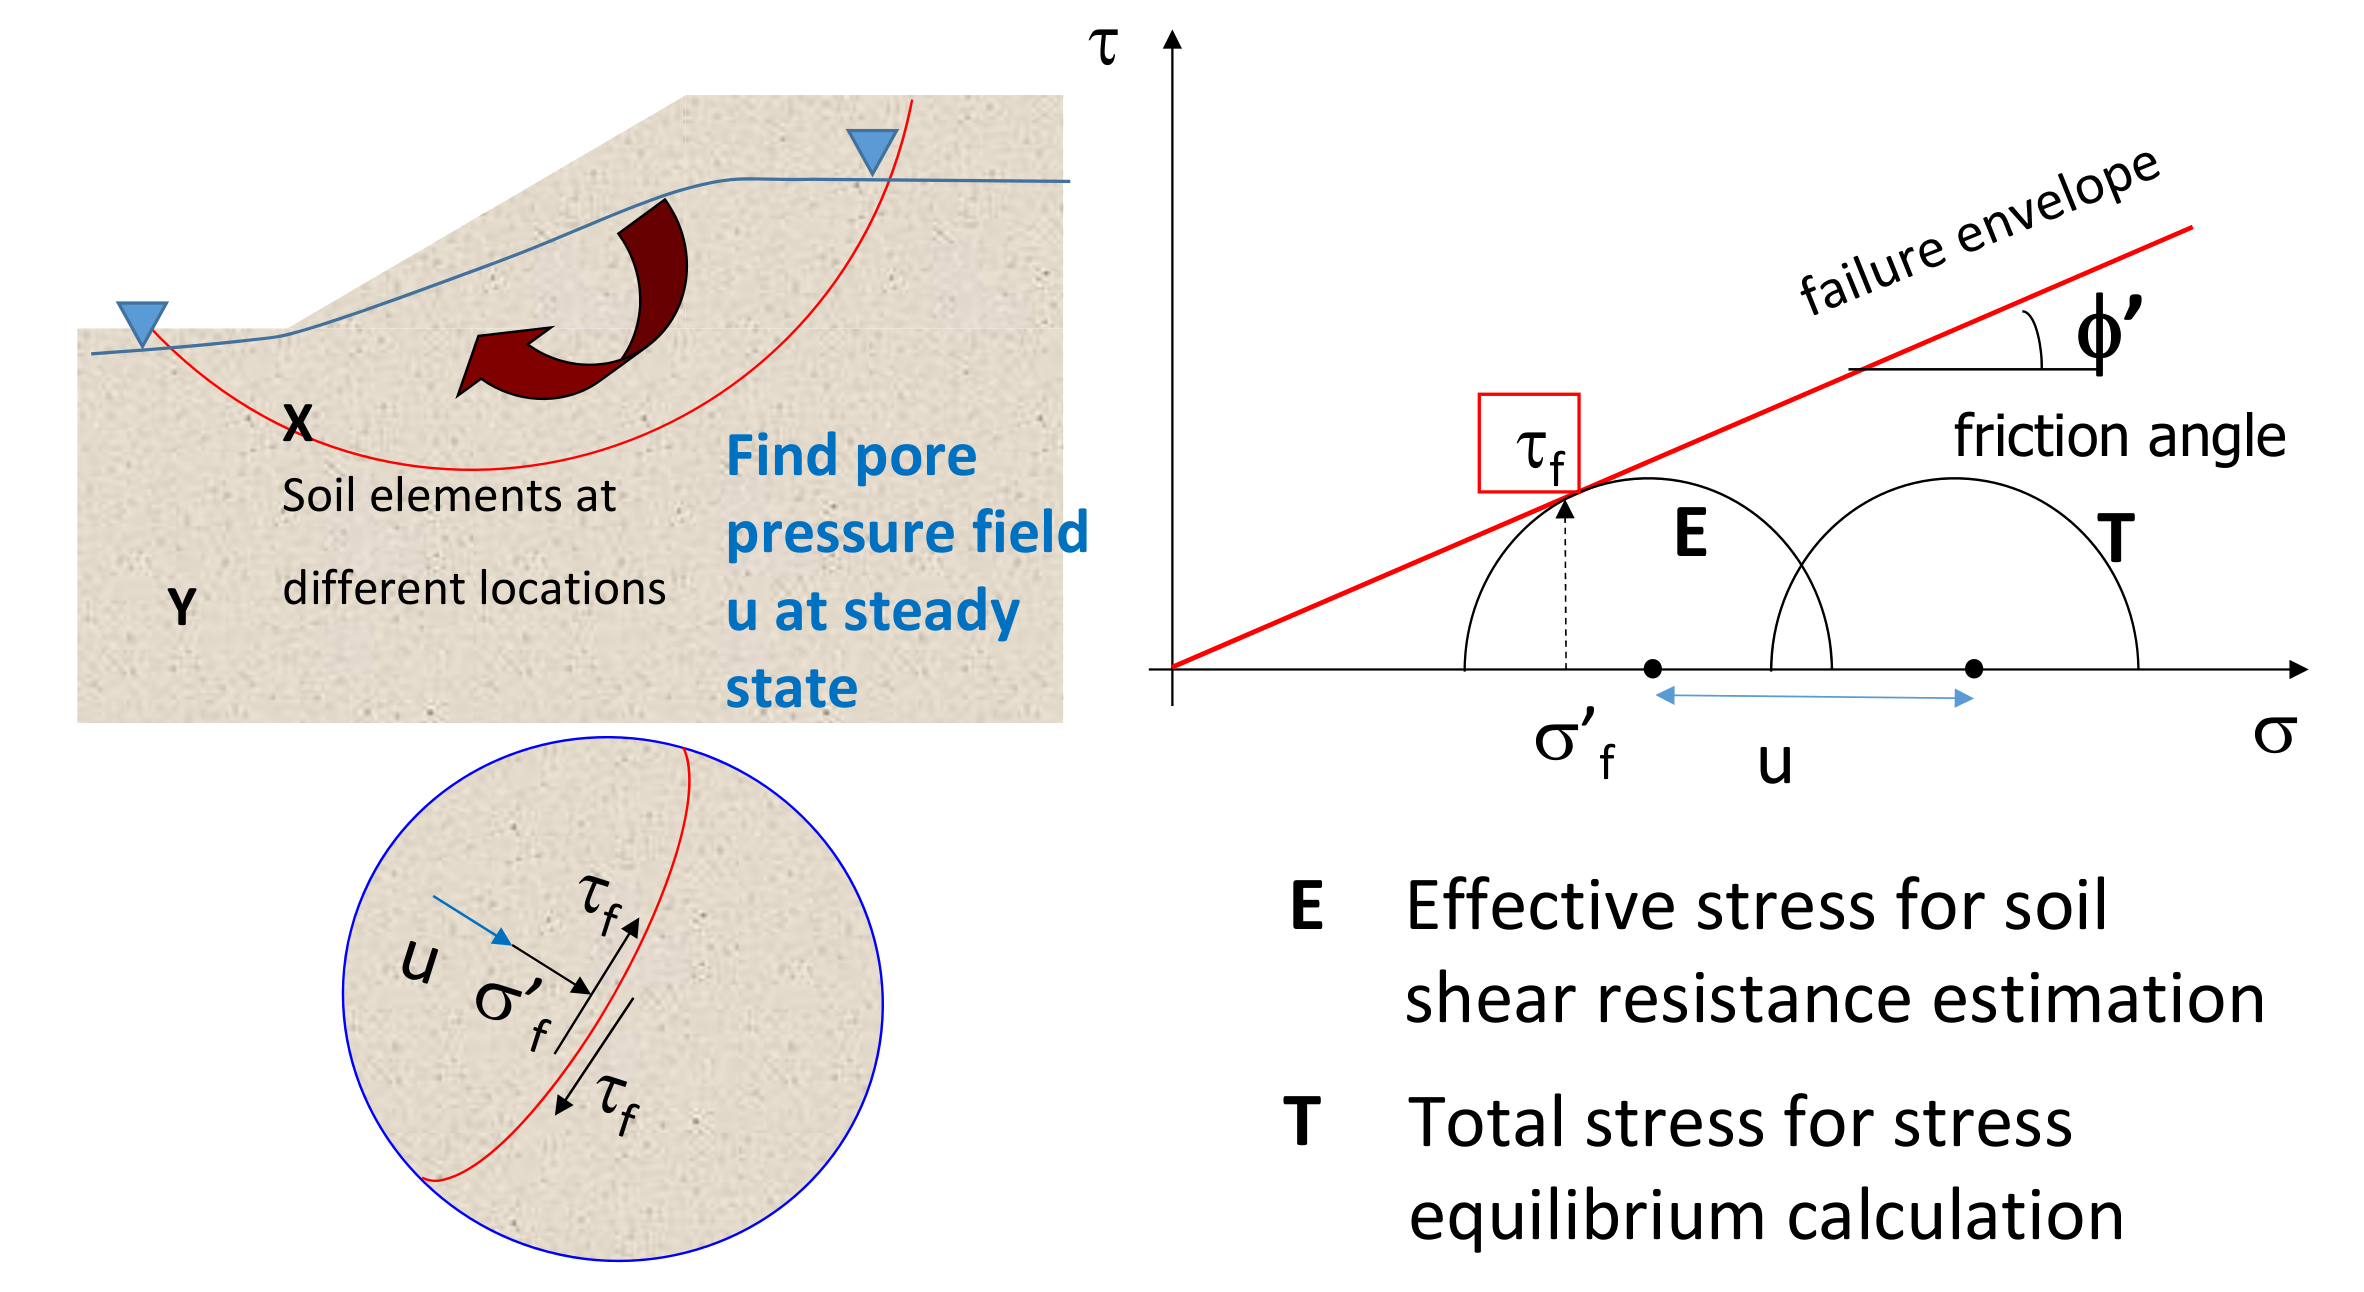
\includegraphics[width=\textwidth]{figs/saturated-slope.png}
\end{figure}
}
\mode<handout>{
\begin{figure}[ht]
\centering
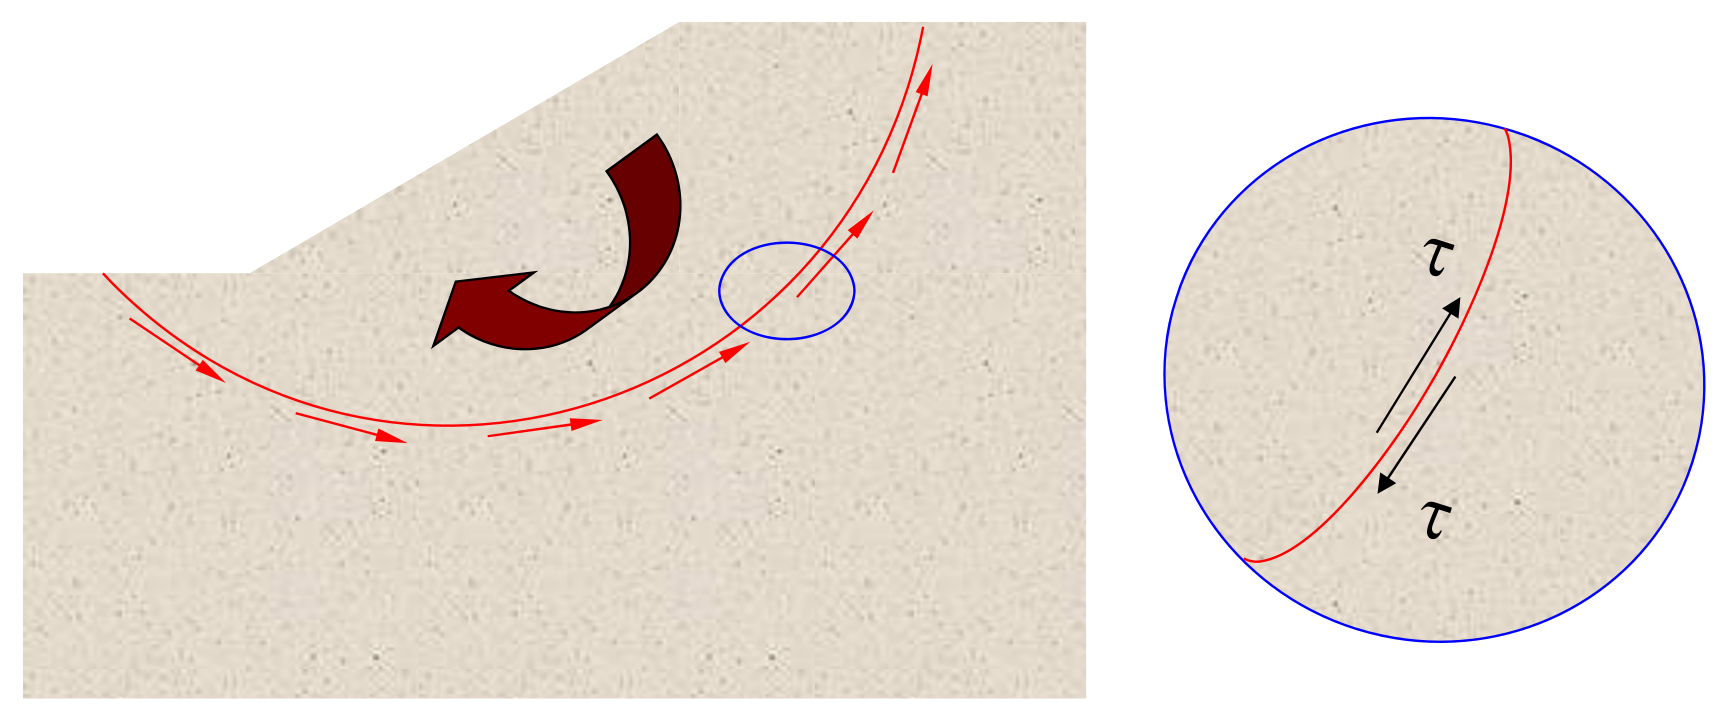
\includegraphics[width=0.9\textwidth]{figs/shear-failure-plane.png}
\end{figure}
}
\end{frame}

%------------------------------------------------
\begin{frame}
\frametitle{Saturated slope (total stress = effective stress + PWP)}
\textbf{Undrained conditions} ‐ (total stress approach) – Use ``\textit{total‐stress based}''
shear strength ($s_u$) to find the overall stability (based on total stress
equilibrium).
\mode<beamer>{
\begin{figure}[ht]
\centering
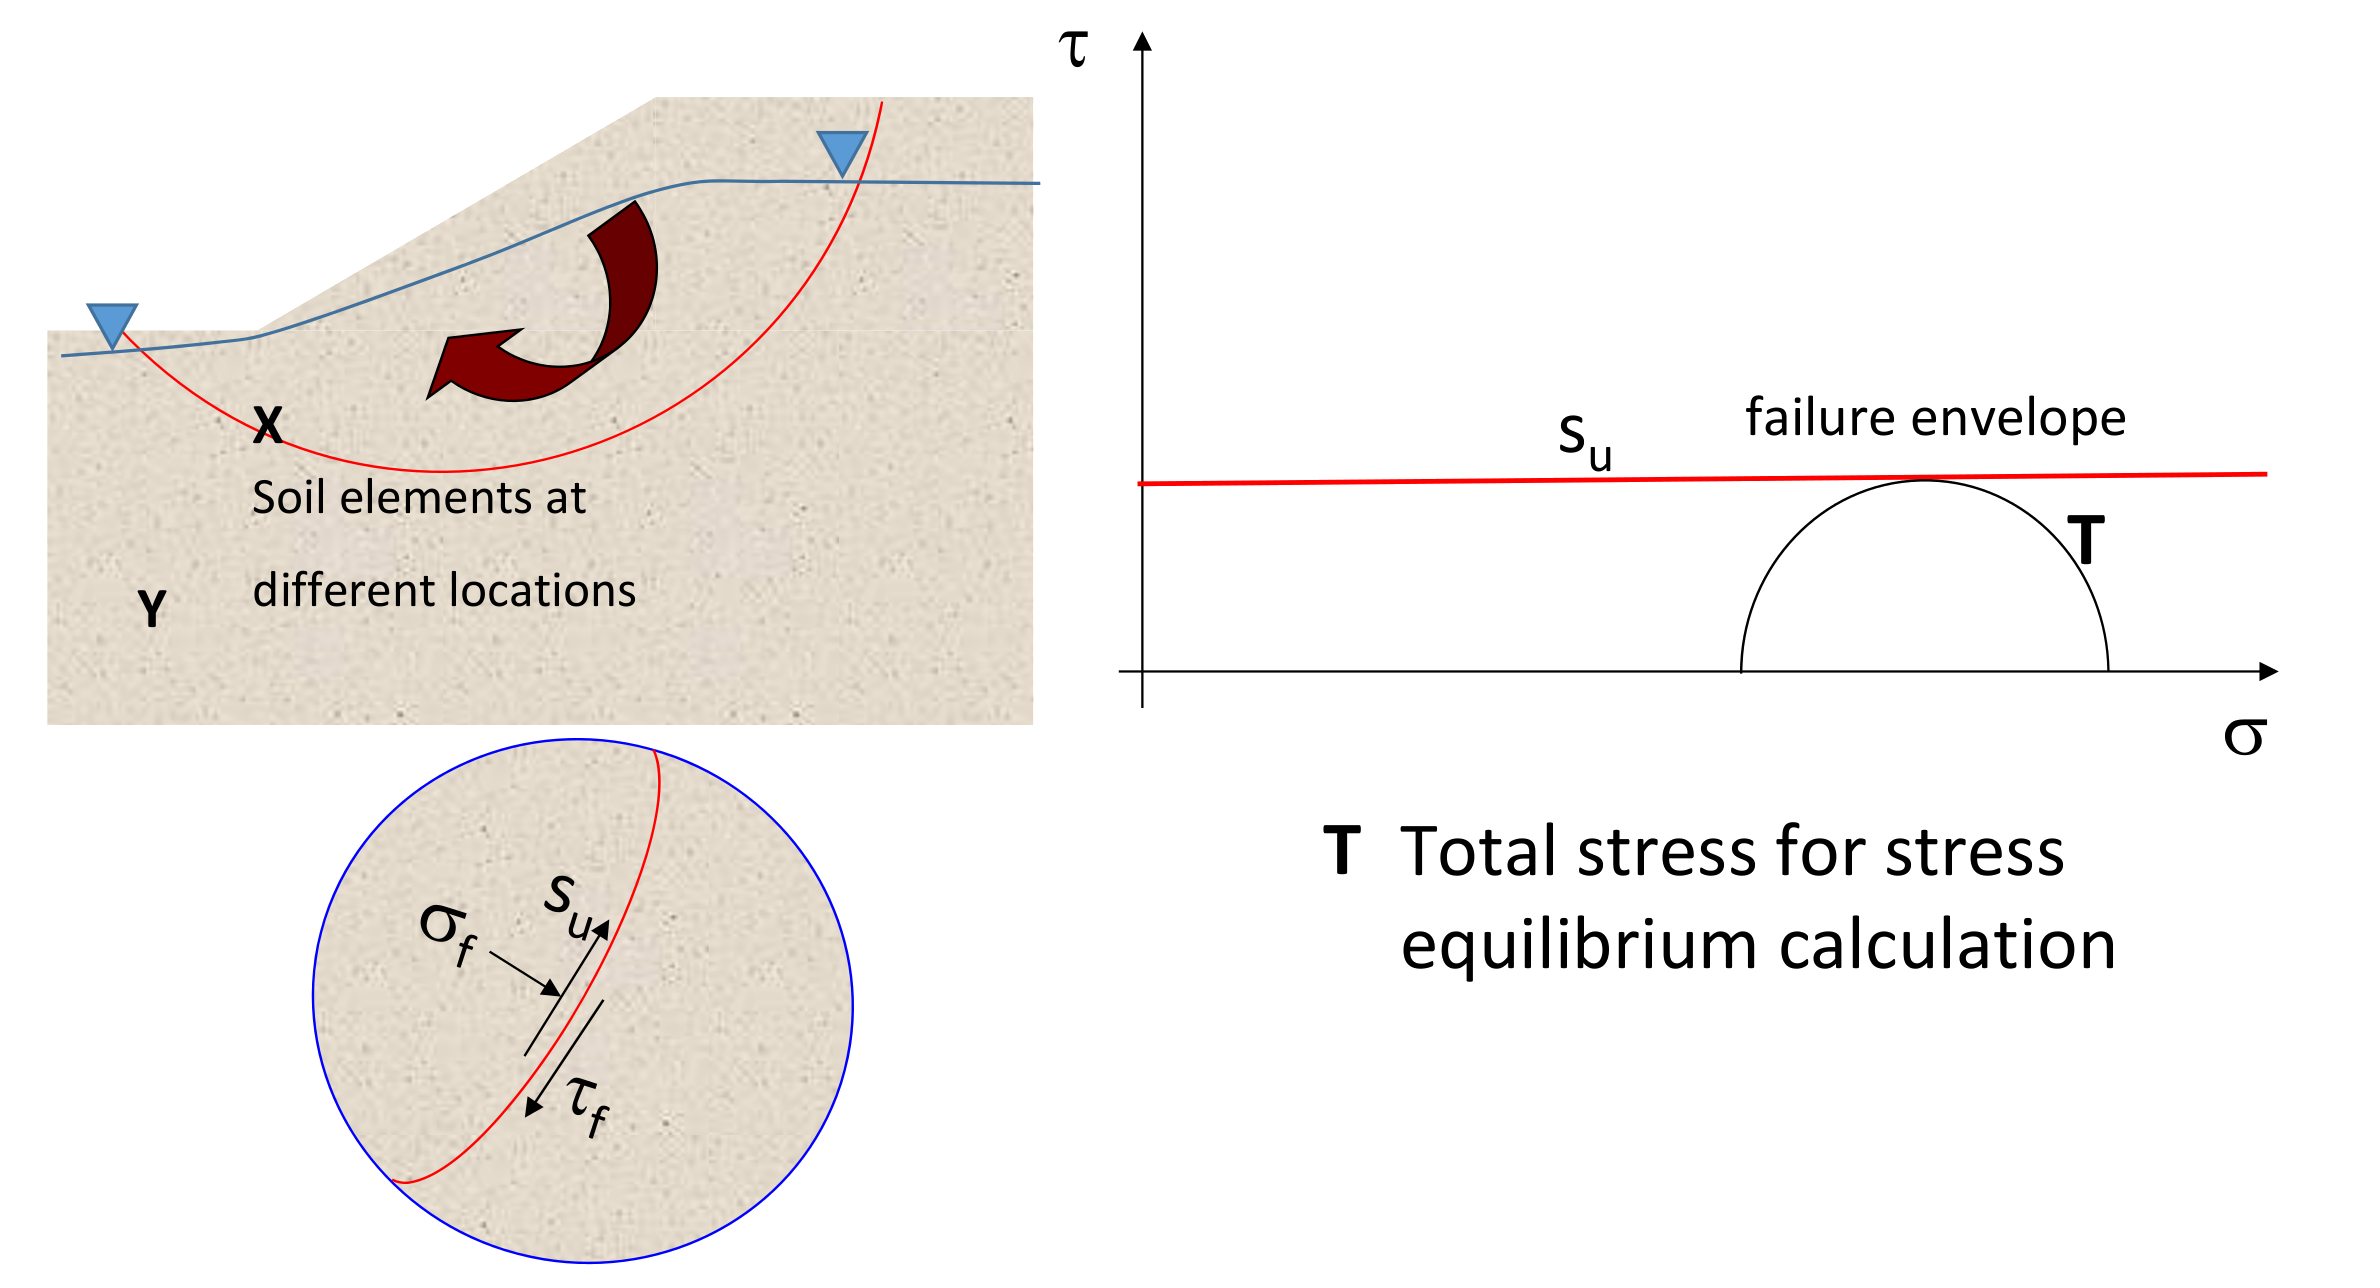
\includegraphics[width=\textwidth]{figs/saturated-undrained.png}
\end{figure}
}
\mode<handout>{
\begin{figure}[ht]
\centering
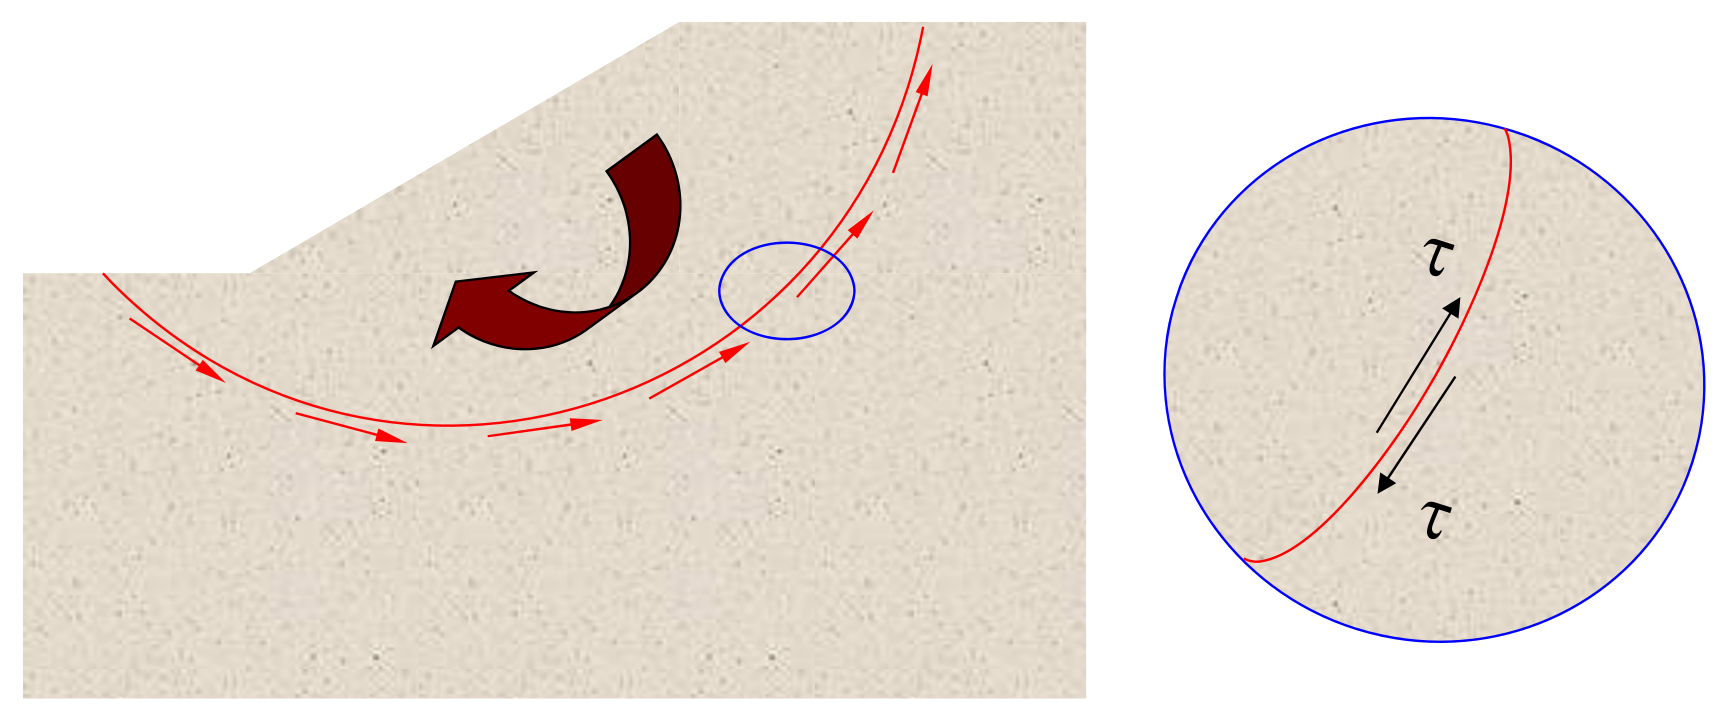
\includegraphics[width=0.9\textwidth]{figs/shear-failure-plane.png}
\end{figure}
}
\end{frame}

%------------------------------------------------
\begin{frame}
\frametitle{Saturated slope (total stress = effective stress + PWP)}
\textbf{Undrained conditions} ‐ (Effective stress approach‐not common) ‐ need to
compute the pore pressure (including excess pore pressure) field and then
evaluate ``\textit{effective stress ‐based}'' shear strength to find the overall stability
(based on total stress equilibrium).
\mode<beamer>{
\begin{figure}[ht]
\centering
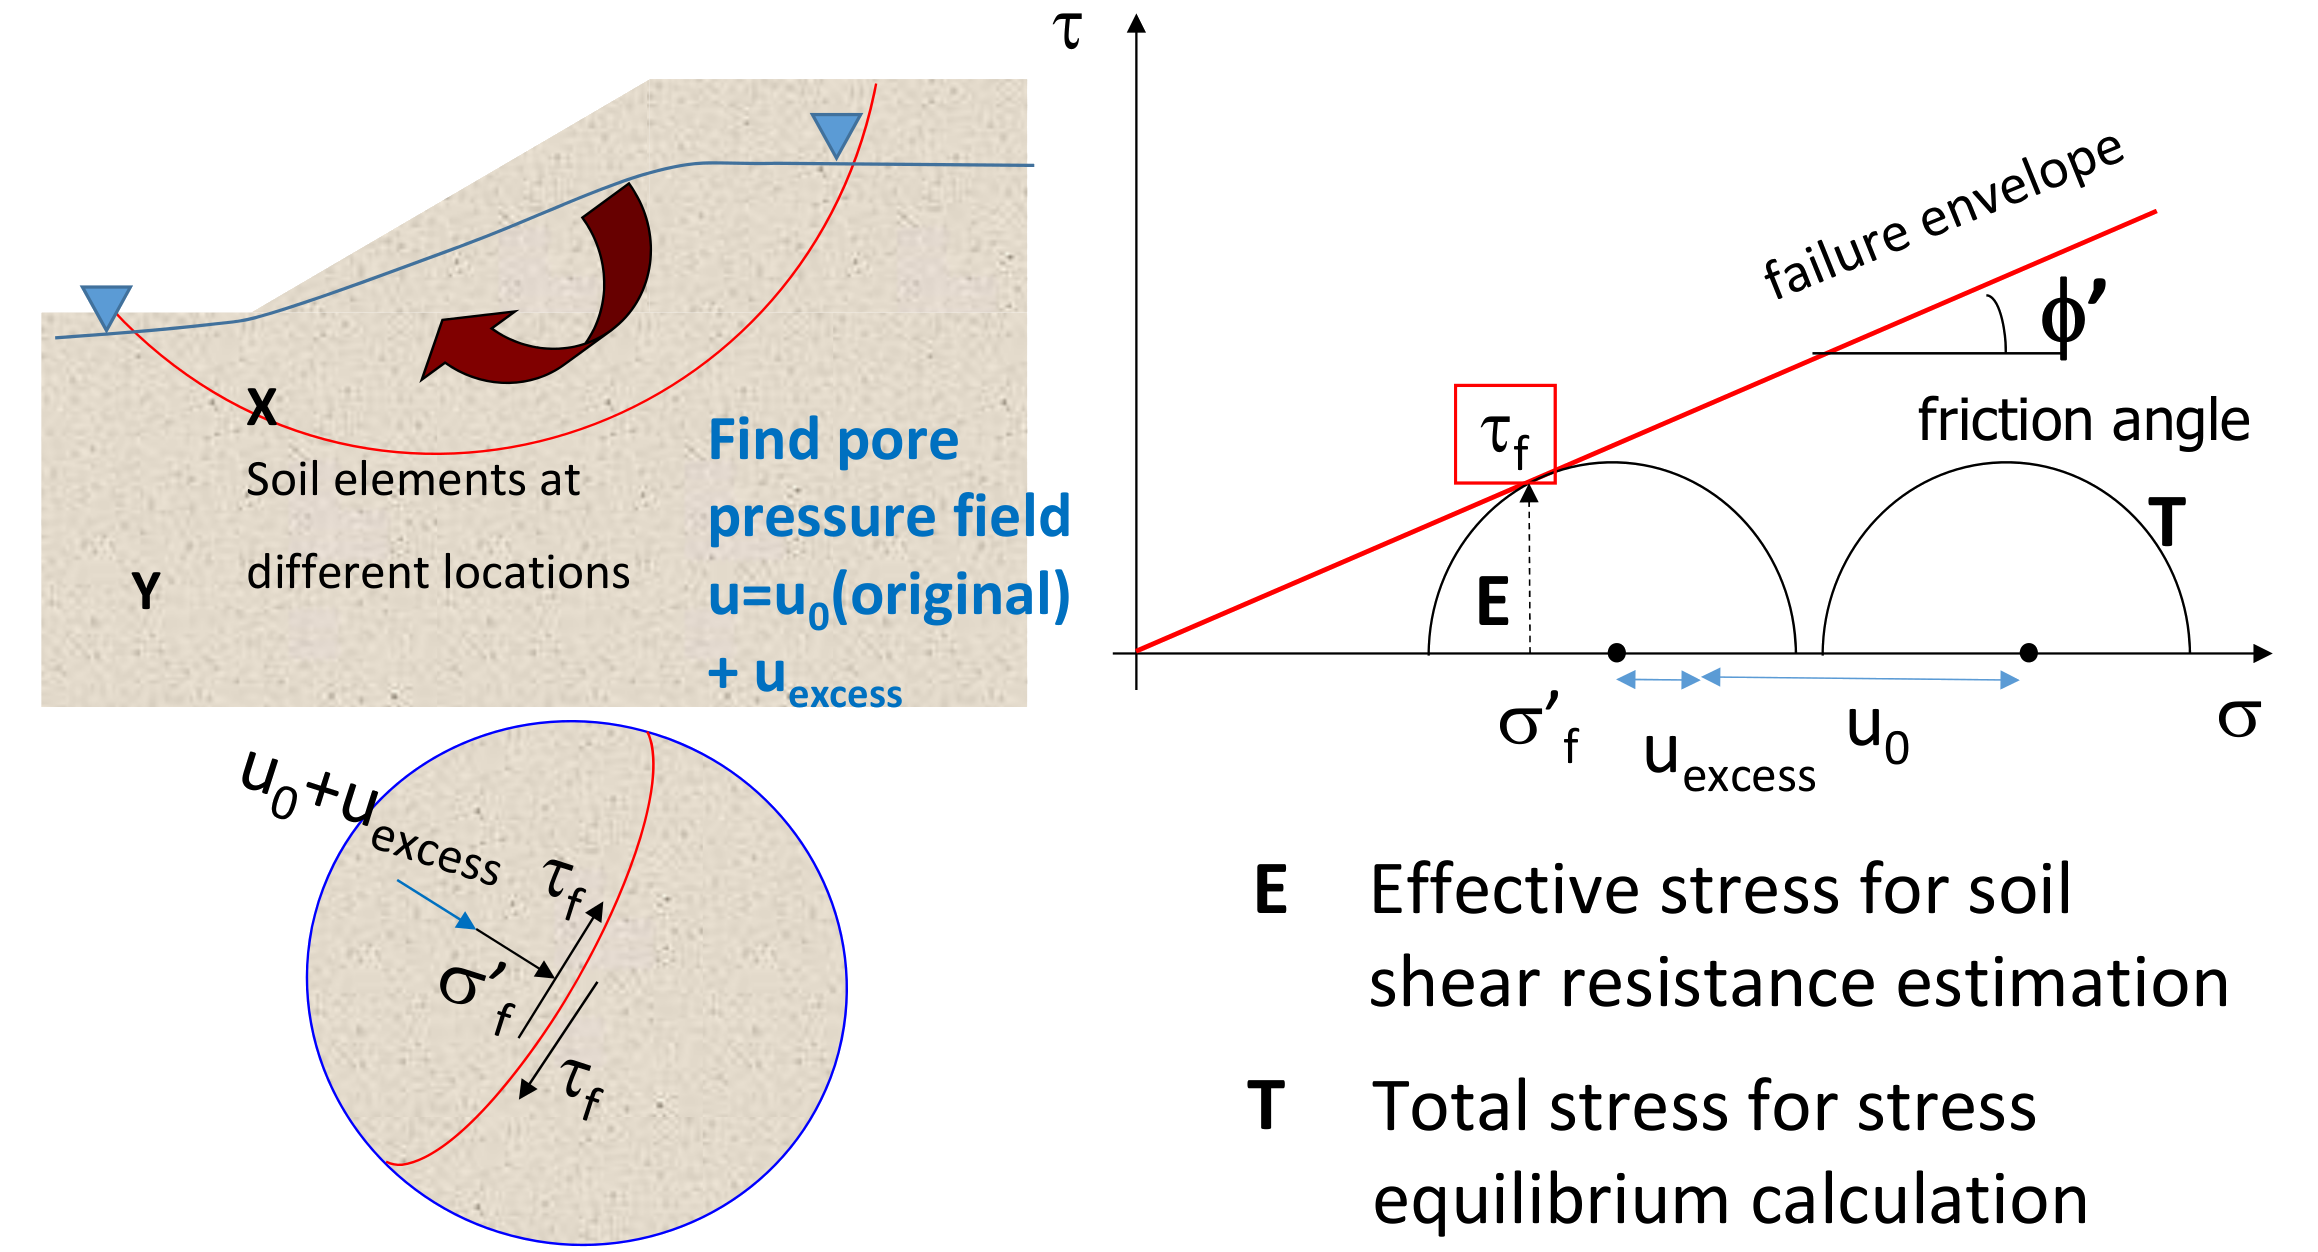
\includegraphics[width=\textwidth]{figs/undrained-effective-stress.png}
\end{figure}
}
\mode<handout>{
\begin{figure}[ht]
\centering
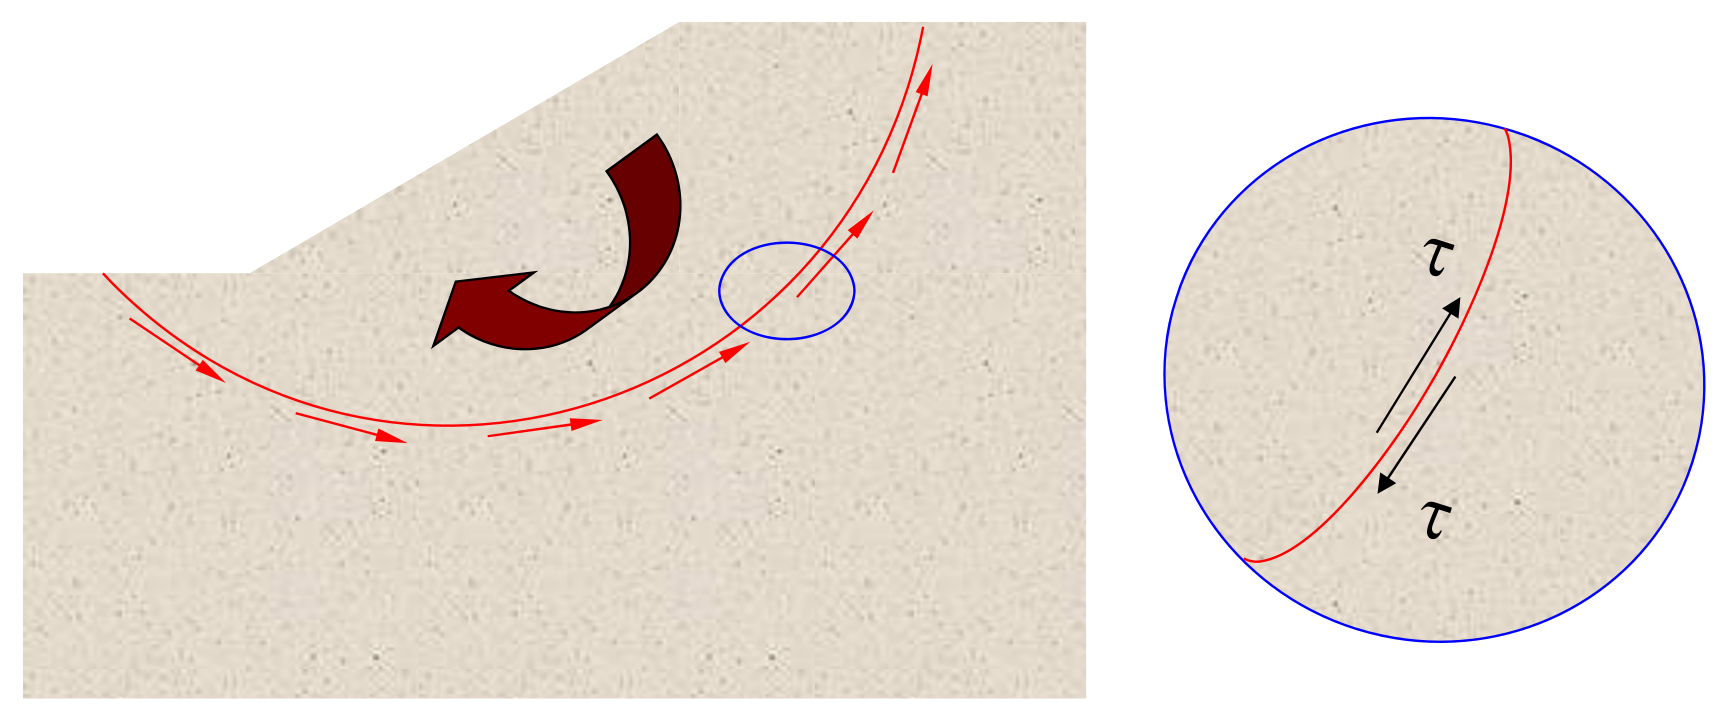
\includegraphics[width=0.9\textwidth]{figs/shear-failure-plane.png}
\end{figure}
}
\end{frame}

%------------------------------------------------
\begin{frame}
\frametitle{Infinite slopes}
\begin{figure}[ht]
\centering
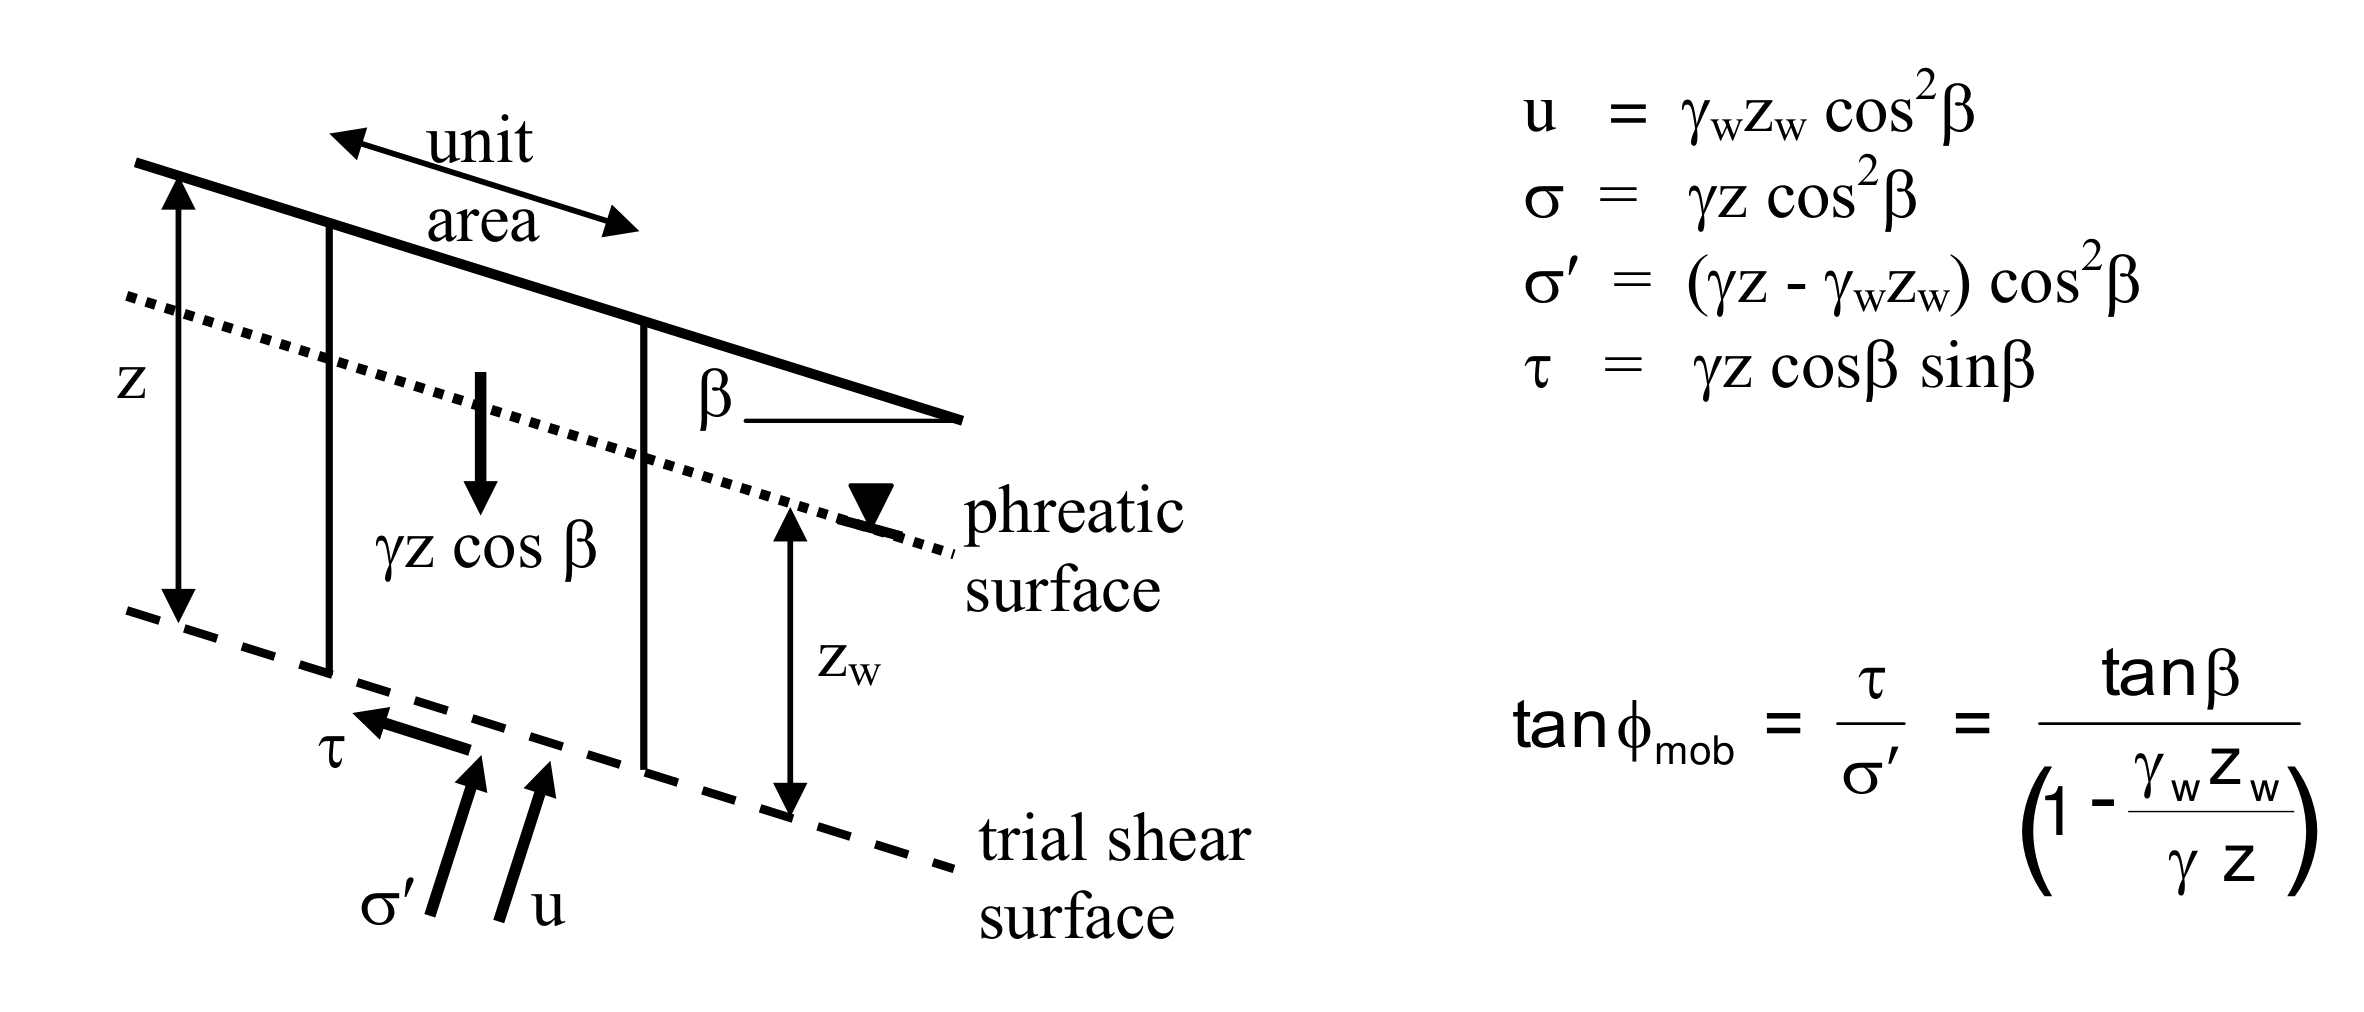
\includegraphics[width=0.9\textwidth]{figs/infinite-slope.png}
\end{figure}
Soil fails when (dry): \mode<beamer>{$ \beta = \phi_{\mathrm{mob}}$}
Soil fails when (submerged): \mode<beamer>{$ \beta = \phi_{\mathrm{mob}}$}
\mode<beamer>{Slope with steady state seepage (drained): $\tan(\beta) = (1 – \gamma_w /\gamma) \tan(\phi_{\mathrm{mob}})$}
\end{frame}

%------------------------------------------------
\begin{frame}
\frametitle{Undrained infinite slope (total stress approach)}
\begin{figure}[ht]
\centering
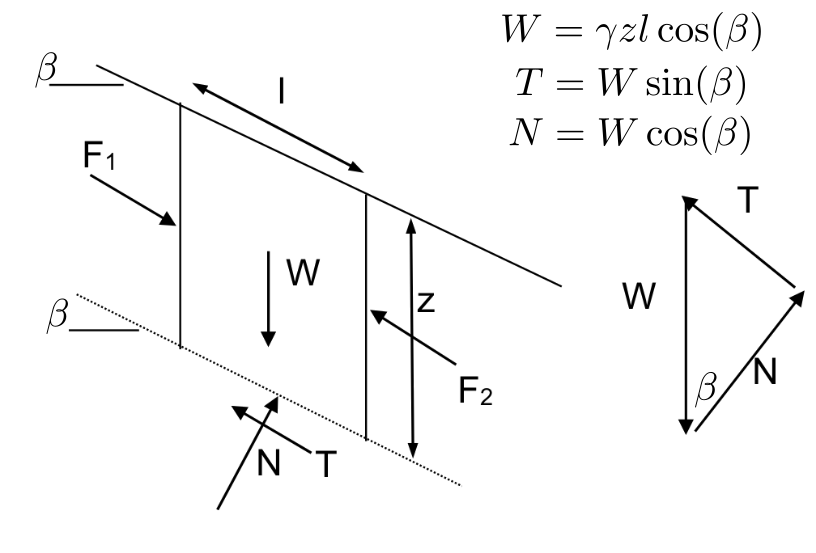
\includegraphics[width=0.8\textwidth]{figs/undrained-infinite-slope.png}
\end{figure}
But also the shear stress: \mode<beamer>{$ T =  s_u l$. The slope failure is governed by $s_u$ profile (with depth).}
\end{frame}


%------------------------------------------------
\begin{frame}
\frametitle{Infinite slope: Summary}
\begin{figure}[ht]
\centering
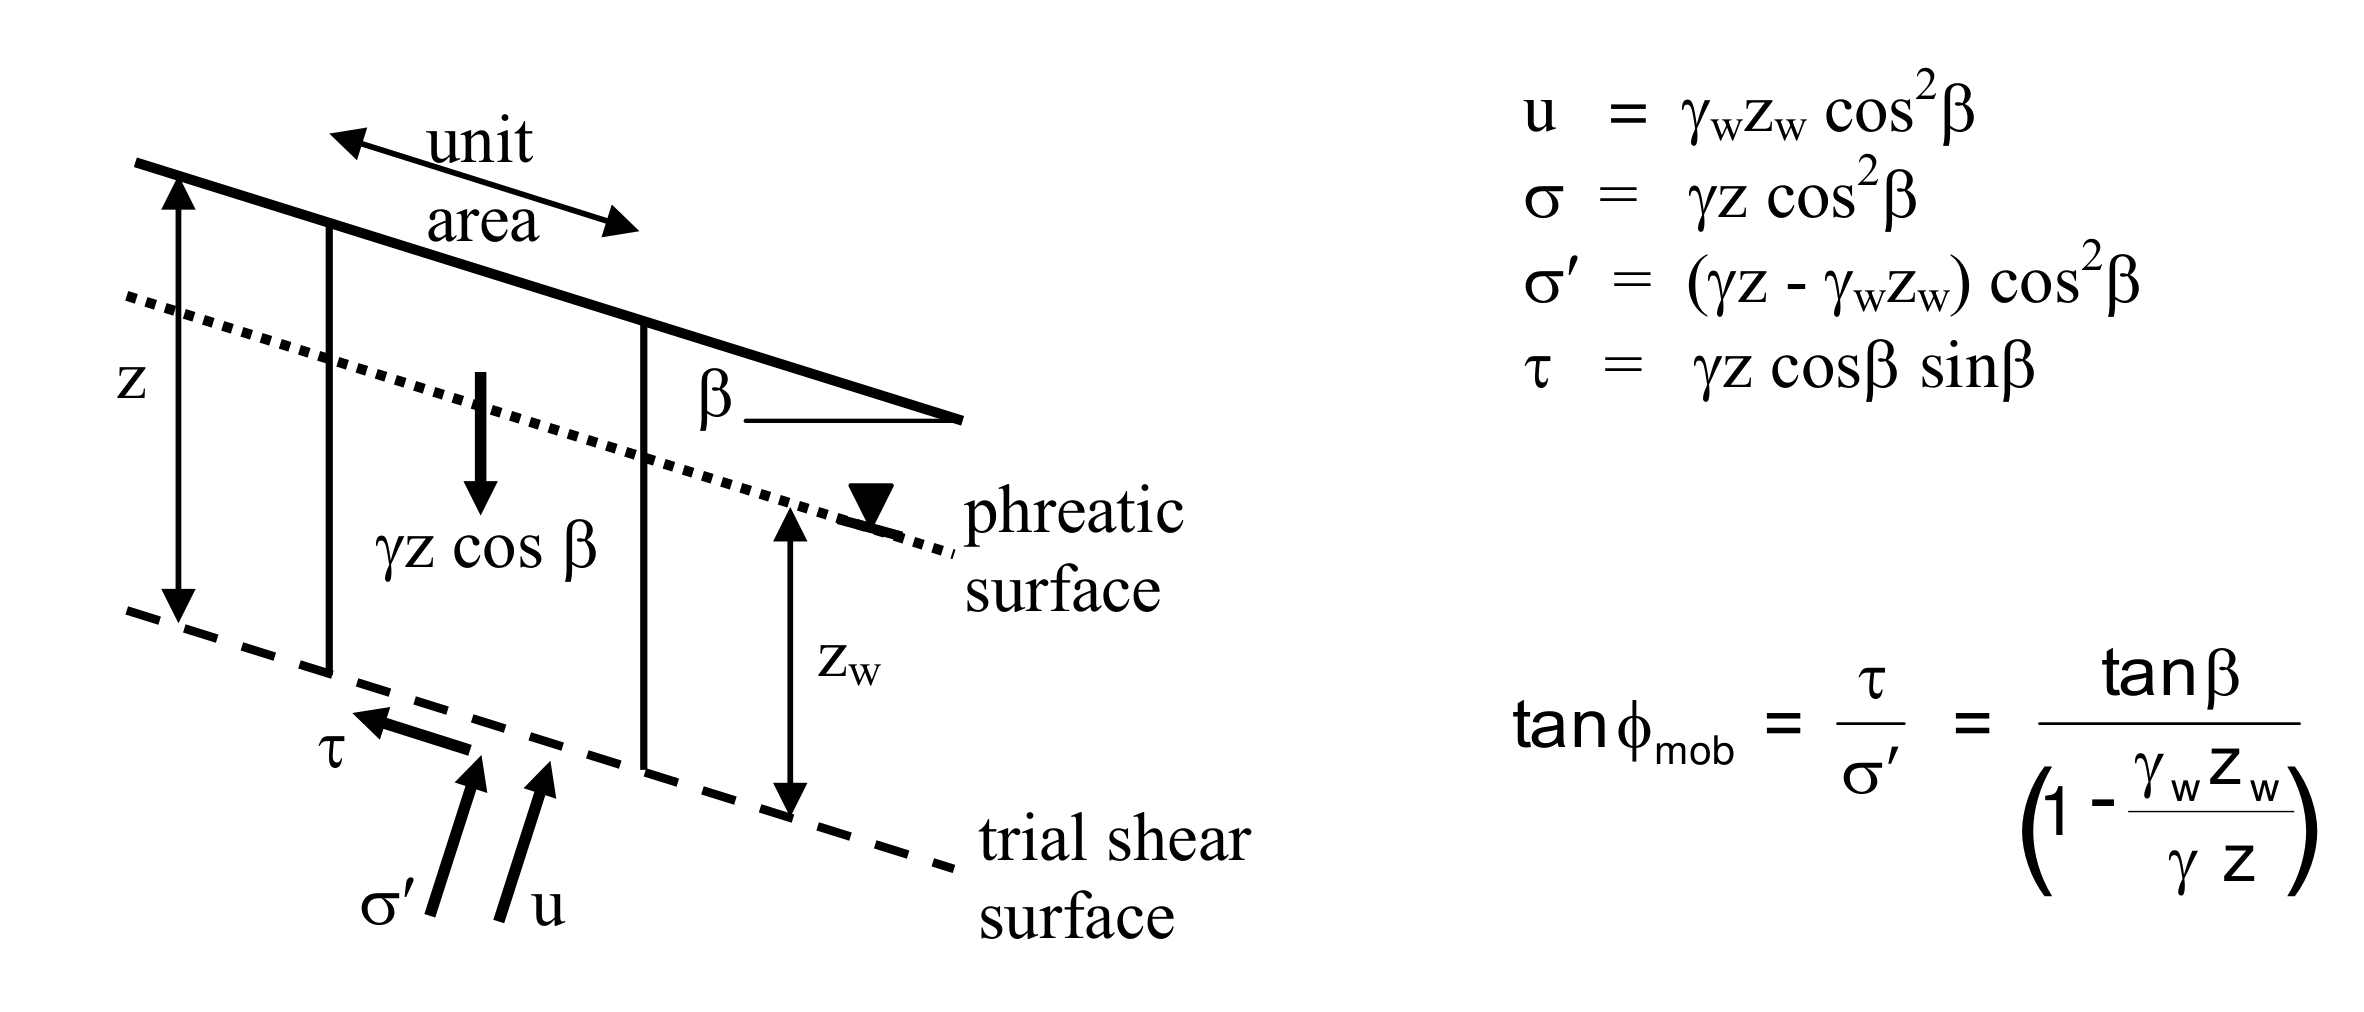
\includegraphics[width=0.6\textwidth]{figs/infinite-slope.png}
\end{figure}
\begin{enumerate}
\item Factor of Safety = resistance / driving
\item Dry FoS = $\tan(\phi_{\mathrm{mob}})/\tan(\beta)$
\item Submerged FoS = $\tan(\phi_{\mathrm{mob}})/\tan(\beta)$
\item Undrained FoS = $2 s_u / \gamma z \sin(2 \beta)$
\item Steady state seepage FoS = $(1 - \gamma_w/ \gamma) \tan(\phi_{\mathrm{mob}})/\tan(\beta)$ where the water table is located at the slope surface
\end{enumerate}
\end{frame}


\end{document}
